%%%%%%%%%%%%%%%%%%%%%%%%
% Sample use of the infthesis class to prepare an MSc thesis.
% This can be used as a template to produce your own thesis.
% Date: June 2019
%
%
% The first line specifies style options for taught MSc.
% You should add a final option specifying your degree.
% *Do not* change or add any other options.
%
% So, pick one of the following:
% \documentclass[msc,deptreport,adi]{infthesis}     % Adv Design Inf
\documentclass[msc,deptreport,ai]{infthesis}      % AI
% \documentclass[msc,deptreport,cogsci]{infthesis}  % Cognitive Sci
% \documentclass[msc,deptreport,cs]{infthesis}      % Computer Sci
% \documentclass[msc,deptreport,cyber]{infthesis}   % Cyber Sec
% \documentclass[msc,deptreport,datasci]{infthesis} % Data Sci
% \documentclass[msc,deptreport,di]{infthesis}      % Design Inf
% \documentclass[msc,deptreport,inf]{infthesis}     % Informatics
%%%%%%%%%%%%%%%%%%%%%%%%

%\documentclass[msc,deptreport]{infthesis} % Do not change except to add your degree (see above).
\usepackage[square, numbers, comma, sort&compress]{natbib}  % Use the "Natbib" style for the
\usepackage{hyperref}
\usepackage[pdftex]{graphicx}
\usepackage{eqparbox}
\usepackage{subfigure}
\usepackage{listings}
\usepackage{xcolor}
\usepackage{pdfpages}

%New colors defined below
\definecolor{codegreen}{rgb}{0,0.6,0}
\definecolor{codegray}{rgb}{0.5,0.5,0.5}
\definecolor{codepurple}{rgb}{0.58,0,0.82}
\definecolor{backcolour}{rgb}{0.95,0.95,0.92}

%Code listing style named "mystyle"
\lstdefinestyle{mystyle}{
  backgroundcolor=\color{backcolour},   commentstyle=\color{codegreen},
  keywordstyle=\color{magenta},
  numberstyle=\tiny\color{codegray},
  stringstyle=\color{codepurple},
  basicstyle=\ttfamily\footnotesize,%\fontsize{8}{8}\selectfont\ttfamily,%
  breakatwhitespace=false,         
  breaklines=true,                 
  captionpos=b,                    
  keepspaces=true,                 
  numbers=left,                    
  numbersep=5pt,                  
  showspaces=false,                
  showstringspaces=false,
  showtabs=false,                  
  tabsize=2
}

%"mystyle" code listing set
\lstset{style=mystyle}

\begin{document}
\begin{preliminary}

\title{Personalized Educational Game in Human-Agent Systems}

\author{Yibin Xia}

\abstract{Due to technology's rapid development, people live under the growing impact of IoT devices. While the IoT ecosystem could bring convenience, the potential privacy threats are also non-negligible, especially for leaking sensitive personal data. There have been many related works focusing on solving privacy issues in the area of mobile apps and IoT devices. In this project, we designed an educational game to help people better understand their privacy preferences and learn more about IoT devices. Following the ethics rules, we conducted a user study to evaluate the game and the system's usability. The results indicate that our project was successful and achieved our aims and educational tasks. This project also provides insights to design a better system for analyzing privacy preferences and educational purposes in the future.}

\maketitle

\section*{Acknowledgements}
Firstly, I want to gratefully thank my supervisor Nadin Kokcyian. Guided by her weekly patient support and professional suggestions, I overcame many obstacles and finally compete this project which made me feel honorable. This is a precious experience for me in my MSc study life and future career.

Secondly, I want to appreciate the University of Edinburgh, which offered me a position to study in such a beautiful environment with abundant resources. I gained a lot of useful knowledge through various courses.

Additionally, I want to thank my participants who spend their time to help me with my project by completing the game and provide feedback, which is really helpful in the evaluation study of my project.

Finally, I want to thank my family, who provided me with financial support, and my cat, who kept me company when I struggled.

\clearpage

{\centering\section*{Declaration}}
I declare that this thesis was composed by myself, that the work contained herein is
my own except where explicitly stated otherwise in the text, and that this work has not
been submitted for any other degree or professional qualification except as specified.

~\\
~\\
\flushright
(\textit{Yibin Xia})


\tableofcontents
\end{preliminary}

\chapter{Introduction}

% The preliminary material of your report should contain:
% \begin{itemize}
% \item
% The title page.
% \item
% An abstract page.
% \item
% Optionally an acknowledgements page.
% \item
% The table of contents.
% \end{itemize}

% As in this example \texttt{skeleton.tex}, the above material should be
% included between:
% \begin{verbatim}
% \begin{preliminary}
%     ...
% \end{preliminary}
% \end{verbatim}
% This style file uses roman numeral page numbers for the preliminary material.

% The main content of the dissertation, starting with the first chapter,
% starts with page~1. \emph{\textbf{The main content must not go beyond page~40.}}

% The report then contains a bibliography and any appendices, which may go beyond
% page~40. The appendices are only for any supporting material that's important to
% go on record. However, you cannot assume markers of dissertations will read them.

% You may not change the dissertation format (e.g., reduce the font
% size, change the margins, or reduce the line spacing from the default
% 1.5 spacing). Over length or incorrectly-formatted dissertations will
% not be accepted and you would have to modify your dissertation and
% resubmit.  You cannot assume we will check your submission before the
% final deadline and if it requires resubmission after the deadline to
% conform to the page and style requirements you will be subject to the
% usual late penalties based on your final submission time.



\section{Motivation}

Due to the rapid development of technology in recent years, there has been a trend that more and more people live under the influence of IoT devices \cite{Kumar}. As its name suggests, the Internet of Things (IoT) is a vast network that connects various kinds of information sensing and collecting devices to build interconnections between humans, intelligent agents, and edge devices \cite{IoT}. Invented by Bill Gates, the concept of IoT has been mentioned long since 1995. While in these days, IoT devices such as air quality monitors, voice controllers, smart speakers, etc., are gradually involved in people's daily lives and have become the most popular intelligent agents \cite{IoTdevice}.

While the IoT ecosystem could provide convenience to people, it could also bring us privacy issues. For example, a temperature sensor equipped in the kitchen may measure the room temperature, a facial recognition-based payment system equipped in a department store may scan and store customer's facial information, a GPS tracker in a smartwatch may read user's local position. Subsequently, the data collected by the connected IoT device may be shared with other authorities or uploaded to the cloud server without user's awareness. More importantly, the data shared with others are usually sensitive, which generally involves our personal or biometric information. The authorities who collect our data have different purposes. They may use the data for cloud-based big data analysis or do improper things such as illegally leaking the data to third parties without notifying us and such that our privacy rights would be threatened \cite{bigdata}.

In the research of Helen Nissenbaum et al., they pointed out that privacy issues have been one of the most prevalent social issues in the area of digital electronic information technologies, and researchers have concluded that privacy issues are complex and hard to conceptualize \cite{privacy, Daniel}. One of the main reasons behind this is that people usually don't have their privacy preferences in mind, such that they don't know whether to allow or deny when they are facing data collection requested by IoT devices \cite{PMID:25635091}. However, the privacy preference in the IoT ecosystem are complicated because they are changeful under different scenarios. People will face different data collection requests in various situations, which are composed of several factors such as specific location, what kind of data will be collected, the purpose of gathering that data, etc, and those factors are usually complicated and interrelated. Consequently, it would be better for people to learn much more about their privacy preferences when deal with IoT devices.

\section{Project Aim}
\label{section:aim}

To relieve the privacy issues mentioned in the previous section, the first goal of this project aims to develop a personalized educational game for players that can help them better understand their privacy preferences by providing them with customized feedback according to their reactions. Players will face different scenarios simulated in the game, and they are asked to provide reactions to each scenario. The game is implemented with a preference analysis model, which collects players' reactions to each scenario and generates preference analyzing results for them when they have finished the game.

The other goal of this project is to combine studying with fun. Since this is an educational game, we are focusing on how to have fun while study. In addition to the privacy preference analysis model, the game will examine players' basic knowledge about IoT devices through several pop-up quizzes interspersed in each scenario and provide feedback for their performance on the examinations. 

A user study was conducted for the evaluation of this game. The user study includes a game experience questionnaire that evaluates the overall design and gameplay of the educational game, and a form of system usability scale (SUS) to assess the usability and learnability of the system, as well as a summative comment regarding players' privacy preferences.

\section{Report Structure}

The structure of this dissertation is organized as follows:

Chapter 2 will provide some background knowledge and related work about this project which will help better understand the details of the game content and methodology used to implement the game. 

Chapter 3 will illustrate and explain the methodology used for the game, including the underlying logic of how each game level was designed, the algorithm we applied for preference analysis model, and the arrangement of each scenario for privacy questions.

Chapter 4 will firstly introduce the overall design of the game, including the flowchart and the main page interface, and then the design details for each part of the game will be described respectively.

Chapter 5 will dive into the implementations of the game in detailed level, and some techniques with Unity and C\# scripts will also be introduced.

Chapter 6 will be the evaluation and user study of this project, which includes a game experience survey and a further study on analyzing privacy preferences.

Chapter 7 will recapitulate what we have done in this project and make a summation for our project.

% Citations (such as \cite{P1} or \cite{P2}) can be generated using
% \texttt{BibTeX}. For more advanced usage, the \texttt{natbib} package is
% recommended. You could also consider the newer \texttt{biblatex} system.

% These examples use a numerical citation style. You may also use
% (Author, Date) format if you prefer.

\chapter{Backgrounds}

This chapter will explore and briefly summarize some background knowledge and related work of this project. Specifically, we will firstly introduce and give some examples of cases that incorporate video games with studies, and then we will explore some factors which could affect people's preference, and explain some knowledge behind the algorithm we applied in the analysis of privacy preference.

\section{Educational Games}

When referring to video games, the conventional mindset tells us that video games are usually for recreational purposes and have negative impact on studies if addicted to games. However, we would also benefit from video games if we take advantage of them appropriately. Some studies have shown the benefits of incorporating video games into the study environment, illustrating the improvements in problem-solving skills, learning interest, and knowledge acquisition motivation. \cite{unknown, KIM2009800, CHENG2012669}. For example, in the research of Hyungsung et al., a meta-cognitive strategy designed in game-based learning was proved that can effectively increase student's learning performance \cite{KIM2009800}. In addition, another game-based learning system developed by Chung-Ho Su et al. also shows that compared with traditional face-to-face teaching, game-based learning could help students gain more learning motivations. \cite{CHENG2012669}.

Other than the games-based study environment investigated by researchers, there are also many educational games developed by game companies. For a crazy fan of astronomy and astrophysics, he or she must have heard \textbf{Universal Sandbox}, an excellent space simulator equipped with a physics engine that can simulate the real universe and perform any astronomical phenomenon \cite{Universe}. As one of the most representative educational games, many people have acquired much knowledge about the universe and astrophysics through \textbf{Universal Sandbox}. Another famous example of educational game is civilization series. First released in 1991, the civilization series had sold over 33 million copies and attracted more than forty thousand players who are in love with history, politics, and economics \cite{Civilization}.

\section{Factors Impacting Privacy Preference}

In a recent study by Almuhimedi et al., they have an inspirational discovery that people's privacy preferences could be more effectively controlled by using a permission manager app that takes records of users' choices each time they encounter data collection scenarios by IoT devices \cite{Almuhimedi2015}. This study gives us an insight that if we could provide information about what factors could affect people's privacy preferences, we cold help them better control their privacy issues and avoid potential privacy threatens.

In the context of mobile devices and applications, many studies focus on analyzing factors that could impact individuals' privacy expectations by analyzing their comfort level and willingness to share data \cite{Sadeh2008UnderstandingAC, Tsai09whosviewed, Lin12expectationand}. For example, Sadel et al. built a system for users of mobile devices to manage the permissions for sharing users' locations with others, and they pointed out that it is crucial to improve users' awareness in order to protect their privacy \cite{Sadeh2008UnderstandingAC}. Additionally, Tsai et al. investigated factors about the feedback of data being shared, and they concluded that people are more comfortable when they receive adequate feedback \cite{Tsai09whosviewed}. Furthermore, according to the research conducted by Lin et al., the purpose for which an app requests access to sensitive data and the individual expectations about the behaviors of the app could influence individuals' privacy decisions \cite{Lin12expectationand}.

The studies about factors impacting privacy preference are not limited to mobile apps. In the aspect of IoT data collection, Lee and Kobsa conducted two separate studies investigating five factors of privacy data collection, and they concluded that individuals' privacy preferences are highly dependent on the type of IoT devices, such as monitors or cameras. Their studies also indicated that people would feel much uncomfortable if they are monitored by unknown entities or the government \cite{Lee2016UnderstandingUP, Lee2017PrivacyPM}. In addition to the effect of device type, there are two more factors being studied by Lederer et al.: the situation in which the data is being collected and the entity that manages the data. Their results showed that the relative importance of who is collecting the data is much greater than the importance of the situation of data collection \cite{Lederer03whowants}. Based on the previous studies mentioned above, Naeini et al. did research on predicting privacy expectations by conducting a within-subjects survey which collected the privacy preferences of more than one thousand participants on different scenarios. They also used machine learning methods to train a model that can predict people's privacy expectations, and the model achieved an average accuracy of over 80\% on predicting comfort level and over 75\% on predicting allow/deny decisions \cite{Naeini:2017}. 

\section{Statistical Correlation Coefficients}

Similar to the work of Naeini et al., a preference analysis model will be implemented in this project. The model will take factors that impact preference analysis as input and outputs relative importance coefficients for each factor. The group of Naeini et al. construct several generalized linear mixed models (GLMM) which are particularly useful for modeling experiments with multiple parallel scenarios \cite{Naeini:2017}. Besides that, many other machine learning models such as support vector machine (SVM) and logistic regression model are also applicable in this project \cite{Steinwart2008SupportVM, Ng2001OnDV}.

Even though machine learning models are powerful, they cost time for training and data preprocessing, and they also need a large number of the dataset to improve accuracy. Hence it would be handy if typical statistical methods were used. There are three kinds of statistical correlation coefficients usually used to represent the significance levels between each random variable: Kendall rank correlation coefficient (KRCC), Spearman's rank correlation coefficient (SRCC) and Pearson product-moment correlation coefficient (PPMCC). The PPMCC, also known as simple correlation, calculates the coefficients of linear relationship between two random variables \cite{ref1}, while the SRCC, as its name suggests, measures the coefficients of ordinal random variables which are nonlinear \cite{Puka2011}. Both SRCC and KRCC could be used for discrete values, but the only difference between them is that KRCC is not suitable for ordinal variables. Ordinal represents that there is a ranking between random variables such as score ranking, population ranking etc. The value of each random variable doesn't matter its coefficient, but the relative order between each random variable does matter. We adopted SRCC in this project and the specific algorithm will be introduced in chapter 3.

\chapter{Methodology}

In this chapter, we will cover the underlying logic of designing each game level, the arrangement of each scenario for privacy questions, and the algorithm we chose to analyse privacy preference. 



\section{Code Book of Factors Impacting Preferences}
\label{section:code book}

Naeini et al. investigated the importance of eight factors when presented to individuals in combination, and they ranked those factors based on corresponding Bayesian Information Criterion (BIC) values \cite{Naeini:2017}. The lower the BIC values, the higher the significance level for a particular factor. According to those BIC values, we picked up six factors that have the highest significance level: 
\begin{itemize}
    \item Location: Where the data is collected
    \item Device type: What kind of IoT devices cast the data collection request
    \item Purpose: The purpose why the data is collected
    \item Retention time: How long the data will be stored
    \item Shared: Whether the data will be shared with third parties
    \item Benefit: Who will benefit from the data collection
\end{itemize} 


The code book for each factor is shown in table \ref{tab:factors}, which lists the name for those six factors, the code values for different corresponding levels, and the ranking criterion on which to rank those levels. To fit the data into the preference analysis model, we carefully assigned a value for each factor based on different criterion such that the Spearman's rank correlation coefficient could accurately represents the correlation between each factor. The values range from 0 to 1 to omit normalization processes in order to increase calculation speed.

The factor \textbf{Location} is divided into six levels based on the privacy confidentiality of each space. The highest space confidentiality will achieve the highest score and vice versa. We consider that \textit{your home} has the highest space confidentiality, and then \textit{your friend's home}, and so on. This is a quite straightforward and intuitive way to rank the level of confidentiality. We combined the factor \textbf{Device type} and \textbf{Data type} as Naeini et al. did in their research \cite{Naeini:2017} since these two factors are highly correlated. For any specific IoT device, it usually collects a certain type of data. For instance, iris scanner will always collect people's iris information almost without any exception. We evaluated the sensitivity of data collected by IoT devices and assigned a larger value to the device that collects more sensitive data. Those devices that collect biometric data, such as fingerprint scanners and facial recognition systems, were given higher values. In comparison, lower values were given to those devices which detect environmental information, such as temperature sensors.

There are more than thirteen different \textbf{purposes}, and for each specific purpose, the value will be evaluated individually according to the context. Some of the purposes are intended to help data collectors fulfil other aims irrelevant to users, while others intend to provide a better user experience. In general, we will assign lower values to the former and higher values to the latter. There are some cases where data collectors did not provide any reason why they requested to collect data, in which cases values of 0 will be assigned. The ranking criteria for \textbf{Retention time} is quite straightforward. A longer retention time corresponds to a higher value and vice versa. Notably, the value of \textit{unspecified} is lower than that of \textit{not deleted} because we considered that unspecified data retention time is assumed to be a period longer than one year but not forever. For the rest of the two factors, \textbf{Being shared} and \textbf{Benefit}, their codes of levels are binary values; hence either 0 or 1 will be assigned.

\begin{table}[htbp]
\newcommand{\tabincell}[2]{\begin{tabular}{@{}#1@{}}#2\end{tabular}}  %导言区
\vskip 3mm
\begin{center}
\begin{tabular}{ |c|c|c|c|}
\hline
\textbf{Factor name} & \textbf{Levels(code)}& \textbf{Count} & \textbf{Ranking criteria}\\
\hline
Location    &  \tabincell{c}{1. Department store (0)\\ 2. Work (0.2)\\ 3. Library (0.4)\\ 4. Public restroom (0.6)\\ 5. Friend's house (0.8)\\ 6. Home (1)}&  \tabincell{c}{15\\15\\15\\15\\7\\8}& Space confidentiality\\
\hline
Device type & \tabincell{c}{1. Temperature sensor (0)\\ 2. Presence sensor (0.2)\\ 3. Smartwatch (0.5)\\ 4. Smartphone (0.5)\\5. Camera (0.7)\\ 6. Facial recognition (0.9)\\ 7. Fingerprint scanner (1)\\ 8. Iris scanner (1)}&  \tabincell{c}{16\\17\\8\\6\\15\\5\\5\\3}& \tabincell{c}{Sensitivity of data \\which was collected}\\
\hline
Purpose & A-M different specific purpose & N/A &\tabincell{c}{Each specific purpose \\will be analyzed solely}\\
\hline
Retention time & \tabincell{c}{1. Purpose satisfied (0)\\ 2. Week (0.2)\\ 3. Year (0.4)\\ 4. Unspecified (0.8)\\ 5. Not deleted (1)}& \tabincell{c}{14\\14\\15\\16\\15}& The length of time\\
\hline
Being shared & \tabincell{c}{1. Shared(1)\\ 2. Not shared(0)} & \tabincell{c}{24\\51}&Binary value\\
\hline
Benefit & \tabincell{c}{1. User(1)\\ 2. Data collector(0)} & \tabincell{c}{64\\9}&Binary value\\
\hline
\end{tabular}
\caption{List of factors and the level code for different levels of factors, as well as the ranking criteria for which levels are ranked}
\label{tab:factors}
\end{center}
\vskip -3mm
\end{table}

\section{Scenario Arrangement}

As we mentioned in the project aim, one of the goals of this project is to analyse individual's privacy preference in different scenarios. The data collection scenario in this project consists of combinations of six factors listed in table  \ref{tab:factors}, where the factor levels varied. A simple permutation and combination calculation tells us that there are $$6\times8\times13\times5\times2\times2 = 12480$$ possible combinations in a privacy scenario. Fortunately, in the research of Naeini et al. they have well-designed nearly 330 scenarios in which factors are combined in a rational and reasonable way \cite{Naeini:2017}. Based on this scenario dataset, we carefully selected 75 scenarios with all levels of factors evenly distributed such that they share almost the same weight in calculating their correlated coefficients. The number of occurrences each level appeared in 75 scenarios is also showed in table \ref{tab:factors}.

Note that the \textit{smartwatch} and \textit{smartphone} shared the same code value because they collect the same kind of data type, which is \textit{specific position}. Consequently, these devices are considered identical when calculating the correlated coefficients. The same thing also applied to \textit{fingerprint scanner} and \textit{iris scanner} since they all collect biometric information.

\section{Privacy Preference Analysis Model}

When all factors are encoded into ordinal values using the code book in section \ref{section:code book}, we can use the model to calculate the significance levels for these factors. The significance levels are evaluated based on two criterion: decision and comfort level. During the game session, we will present 75 data collection scenarios to players and ask them some privacy questions, including how they feel about the data collection in the described situation and whether they allow or deny it. We then take records of players' responses and use the statistical models to evaluate the significance levels of factors corresponding to the responses.

\begin{table}[htbp]
    \begin{center}
    \begin{tabular}{ |p{.3\textwidth}| p{.7\textwidth}|}
        \hline
        \textbf{Responses} & \textbf{Variable Type}\\
        \hline
        Allow/Deny Decision& Binary: allow(1), deny(0)\\
        \hline
        Comfort Level & Ordinal: Very uncomfortable(1), Uncomfortable(2), Neither comfortable nor uncomfortable(3), Comfortable(4), Very comfortable(5)\\
        \hline
        \end{tabular} 
    \end{center}
    \caption{The variable type of responses to privacy questions}
    \label{tab:responses}
\end{table}

Table \ref{tab:responses} shows the variable type of player's responses that we will record in the game. Decisions on data collections are indicated as binary outcome variables where approving represents one and rejecting represents zero. The variable type for comfort level is also in an ordinal form on a scale from 1 to 5. It is worth noting that the rankings of decisions and comfort levels are in the same direction, which means the higher the rank, the more likely that players are happy with the data collection. For example, the highest ranking in comfort level is 5 (very comfortable). We followed the convention that if people are more comfortable with the data collection, they are more likely to approve the collection request. Although there might be some exceptions, it would be helpful when we present results to players.

We use Spearman's rank correlation coefficient (SRCC) to calculate the correlated coefficients. The formula of SRCC is showed in equation \ref{equation:SRCC}, among which $d_i$ represents the rank difference between two random variables $X_i$ and $Y_i$. It was proven that $r_s$ ranges from -1 to 1, where the sign of $r_s$ represents the monotonic relationship between dependent and independent variables, and the absolute value of $r_s$ indicates the degree of monotonic relationship \cite{Myers}. In other words, there will be a robust negative association between two variables if $r_s$ approaches -1, a strong positive association if $r_s$ approaches 1, and no apparent monotonic association if $r_s$ approaches 0.

\begin{equation}
\label{equation:SRCC}
    r_s = 1- \frac{6\sum_{i=1}^{n}d_i^2}{n(n^2-1)}
\end{equation}

\section{Pop-up Quiz}

To fulfil another goal of this project,  we designed several pop-up quizzes to examine players' knowledge about IoT devices. There will be ten quizzes randomly distributed in 75 scenarios. The structure of the quizzes is as follows. Firstly, players will be presented in a simulated scenario, such as in a department store or a library, and then they are told that a kind of IoT device is trying to collect their data. Players will not be directly told what the device is, but they will be hinted at by side information such as the function or feature of that IoT device. Afterwards, five icons will be randomly generated through a device pool and players are required to select the correct icon that accurately represents the IoT device mentioned in the quiz. We have prepared eleven icons of IoT devices in the device pool: headphone, iris scanner, presence sensor, fingerprint scanner, facial recognition, temperature sensor, personal computer, camera, smartphone, and smartwatch, respectively.

Each quiz will focus only one IoT device. The number of quizzes for different type of IoT devices is showed in table \ref{tab:quiz}. The results control system implemented in the game will records players answers to the quizzes and evaluate their overall performance and accuracy for specific devices to provide tailored feedback to them. More details about the design of results control system as well as the preference analysis model will be introduced in chapter 4.

\begin{table}[htbp]
    \begin{center}
    \begin{tabular}{ |c| c|}
        \hline
        \textbf{Device name} & \textbf{Count}\\
        \hline
        Facial recognition& 1 \\
        \hline
        Presence sensor& 3\\
        \hline
        Iris scanner & 1\\
        \hline
        Fingerprint scanner & 2\\
        \hline
        Camera & 1\\
        \hline
        Temperature sensor & 1\\
        \hline
        Smartphone & 1\\
        \hline
        Total number of quizzes & 10\\
        \hline
        \end{tabular} 
    \end{center}
    \caption{Number of quizzes subject to the type of IoT device}
    \label{tab:quiz}
\end{table}

\chapter{Game design}

In this chapter, we will introduce this project's game design from the overall and detailed perspectives, respectively. The flowchart for the game and some screenshots of the interfaces will be presented.

\section{Overall Design}

The development tool we chose is Unity, a user-friendly 2D and 3D multi-platform game development engine. Unity has been one of the most popular development platforms, with countless free game materials online, including graphic user interfaces, background music and prefabs. When the game was designed initially, considering we needed to show players as many as 75 scenario-based privacy questions along with the pop-up quizzes, it would be extraordinarily time-consuming and impossible to finish in a timely scale if we built up the whole scene for each privacy question, either in 2D or 3D. Hence we changed the idea to build a text-based interactive game. 

\subsection{Flowchart}
Figure \ref{fig:flowchart} shows the flowchart of this game. When the game is started, there are two options: start a new game and load previous save data. We provided a save function that records the players' data so that if players want to suspend the game sessions, they can continue their sessions next time by loading the data files. A tutorial will be shown if it is the first time playing the game. Afterwards, players will proceed to the main page, which connects every game scene. As shown in the flowchart, the six blocks right below the main page block connected by bidirectional arrows represent six different scenario locations, which contain privacy questions and pop-up quizzes. Players can check their personalized feedback for privacy preferences and pop-up quizzes when they finish privacy questions for all six locations. The mini-game and shop scenes could also be accessed from the main page.

\begin{figure}
    \centering
    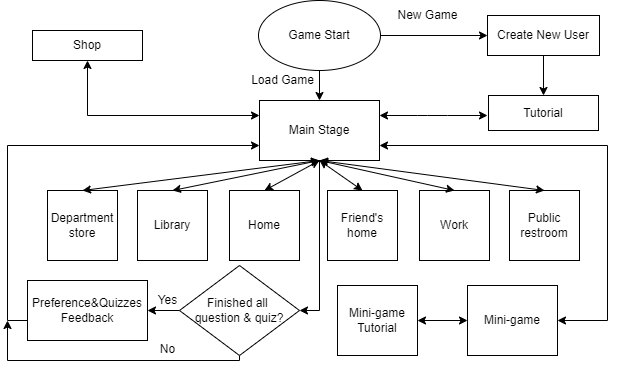
\includegraphics[scale=0.6]{Game Flowchart2.png}
    \caption{The flowchart of the game}
    \label{fig:flowchart}
\end{figure}

\subsection{Main page}
\label{section:main page}

\begin{figure}
    \centering
    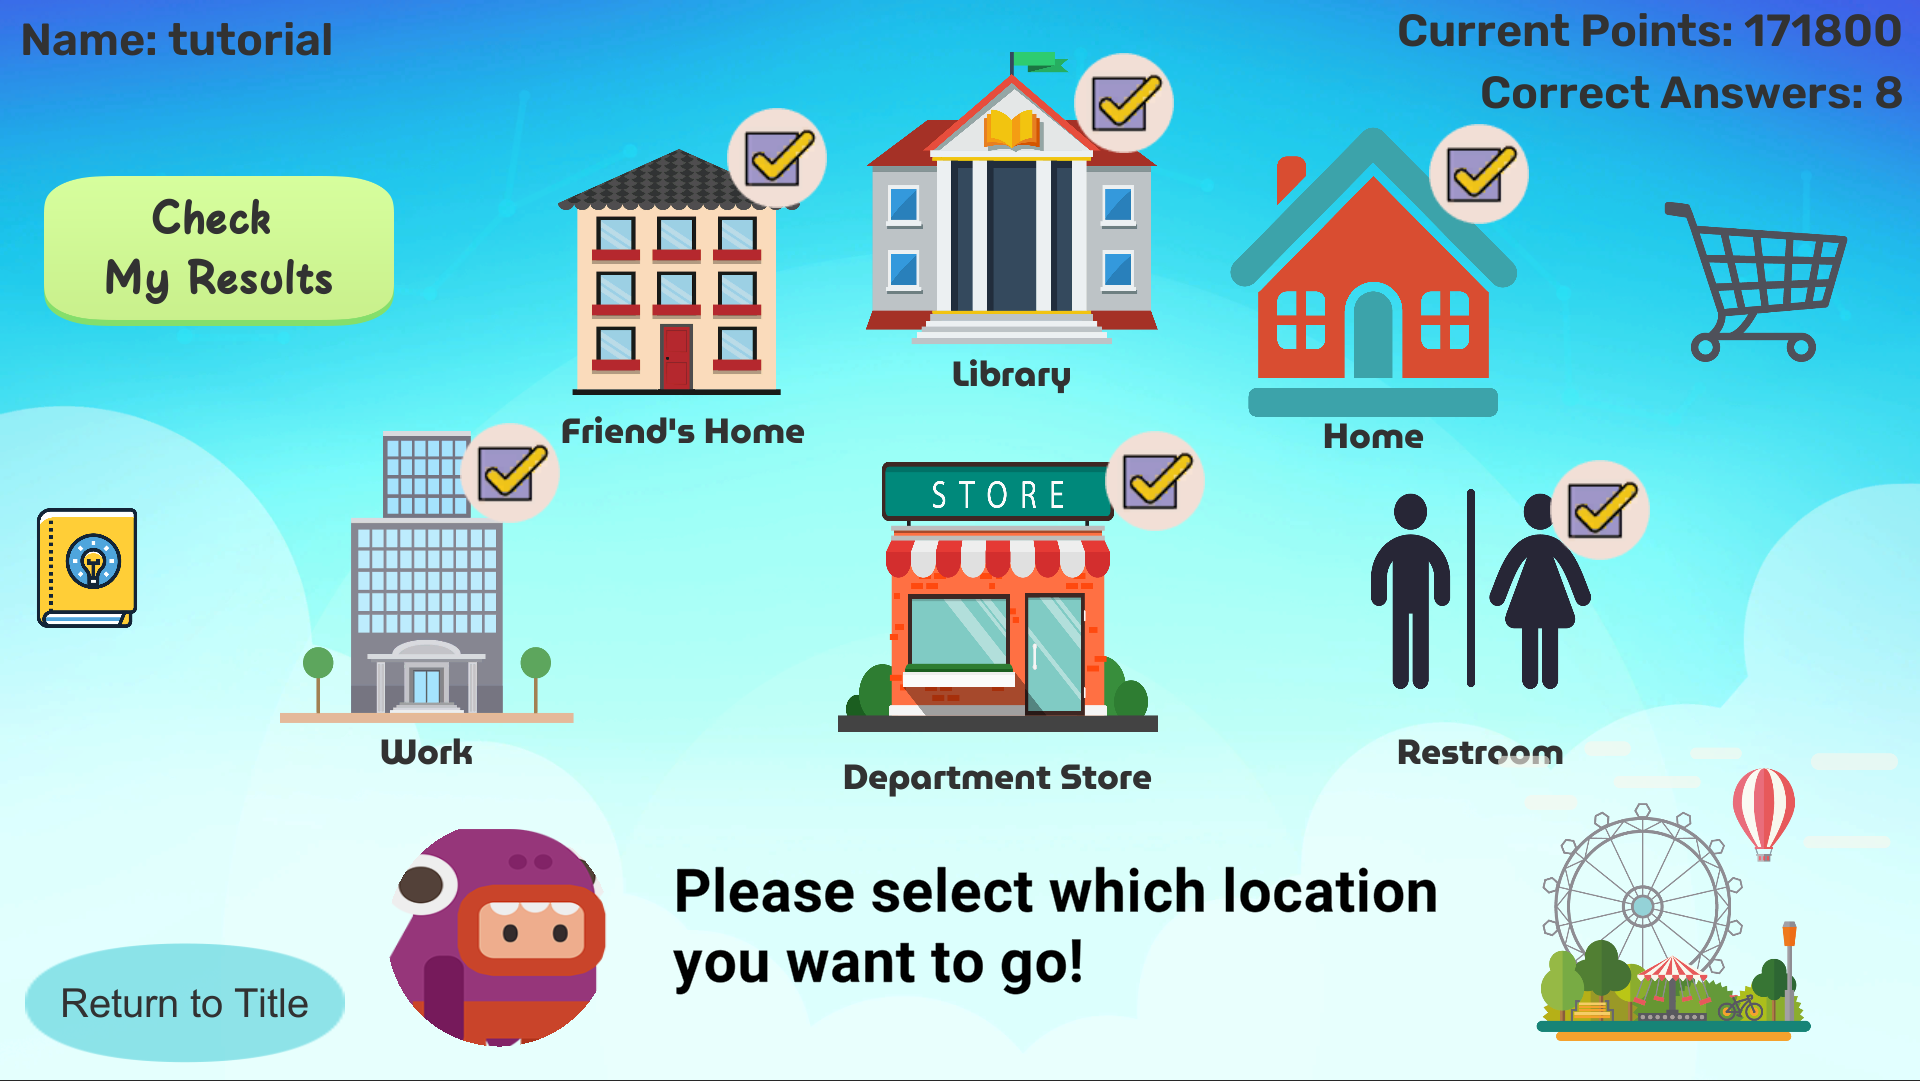
\includegraphics[scale=0.23]{Main Stage.png}
    \caption{The interface of the main page}
    \label{fig:main}
\end{figure}

Figure \ref{fig:main} shows the layout of the main page. The left and right corners indicate players' username, current points earned through the mini-game, and the number of correct answers they got in the pop-up quizzes. The points are used to buy items in the shop, which is shown in the form of a shopping cart icon on the top right side of the interface. The tips icon, a yellow book with a light bulb, is a tutorial button where players could review the game's information and rules if they had skipped the tutorial before.

The middle six icons occupying more than half of the interface are buttons for different locations of privacy questions. Clicking one of the location buttons will direct players to a scene that will include every privacy event that happens at that location. For example, if players click the button tagged as department store, they will face several privacy questions related to the department store. Furthermore, the related IoT devices for pop-up quizzes will also appear in the department store. The reason why we did this is that we want to simulate scenarios as realistic as possible. When players finish all privacy questions and pop-up quizzes on the department store, the corresponding icon will be ticked, and players can proceed to the following location. A green button on the top left side will be available to check their results when all six sites are ticked. The mini-game icon, located on the bottom right, provides an entry to the mini-game which will be introduce in the next section.

\section{Design Details}

In this section, we will introduce the design of this game in detailed level, which consists of several part: introductory pages,  scenario-based privacy questions, pop-up quizzes for IoT devices, mini-game, and results analysis model.

\subsection{Introductory pages}
\label{section:intro}

When players first enter the game, they will be shown some introductory pages which will briefly introduce the game and help them to create their own save file. In the introductory pages, players are asked to input their username, as shown in figure \ref{fig:name}. The system will warn players if the inputted username is too long (over ten characters) or too short (below three characters). The system would also do a comparison search with the database to prevent name conflict. If a player inputs a username that other players already take, the system will also cast a warning text shown in figure \ref{fig:name_c}. 

\begin{figure}[htbp]
\center
\subfigure[name is too short]{
\begin{minipage}[c]{0.48\textwidth} %自行调整,太大的话会自动换行
\centering
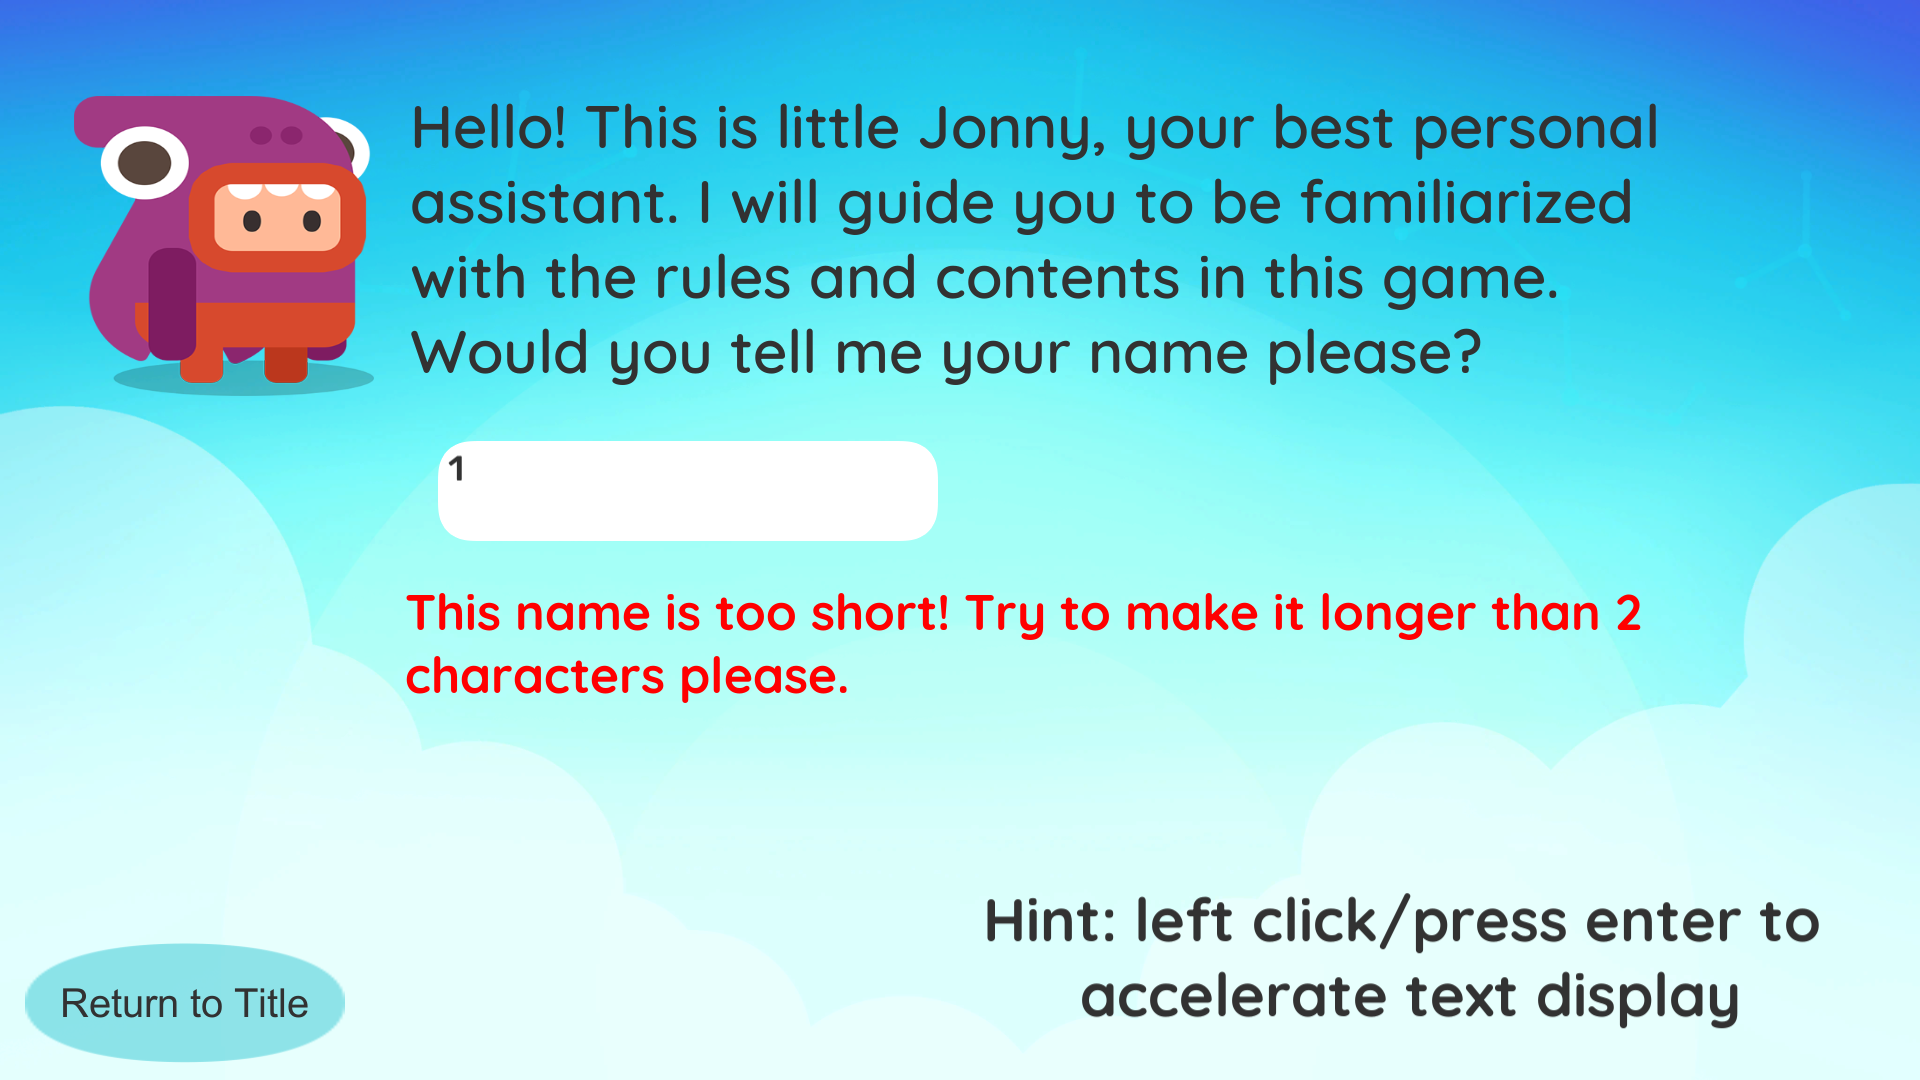
\includegraphics[width=1\textwidth]{Name_a.png}
%width相加大于1时自动换行
%自行调整width \vsapce \hspace
\end{minipage}
}\hspace{-1pt}%调整subfigure的间距
\subfigure[name is too long]{
\begin{minipage}[c]{0.48\textwidth}
\centering
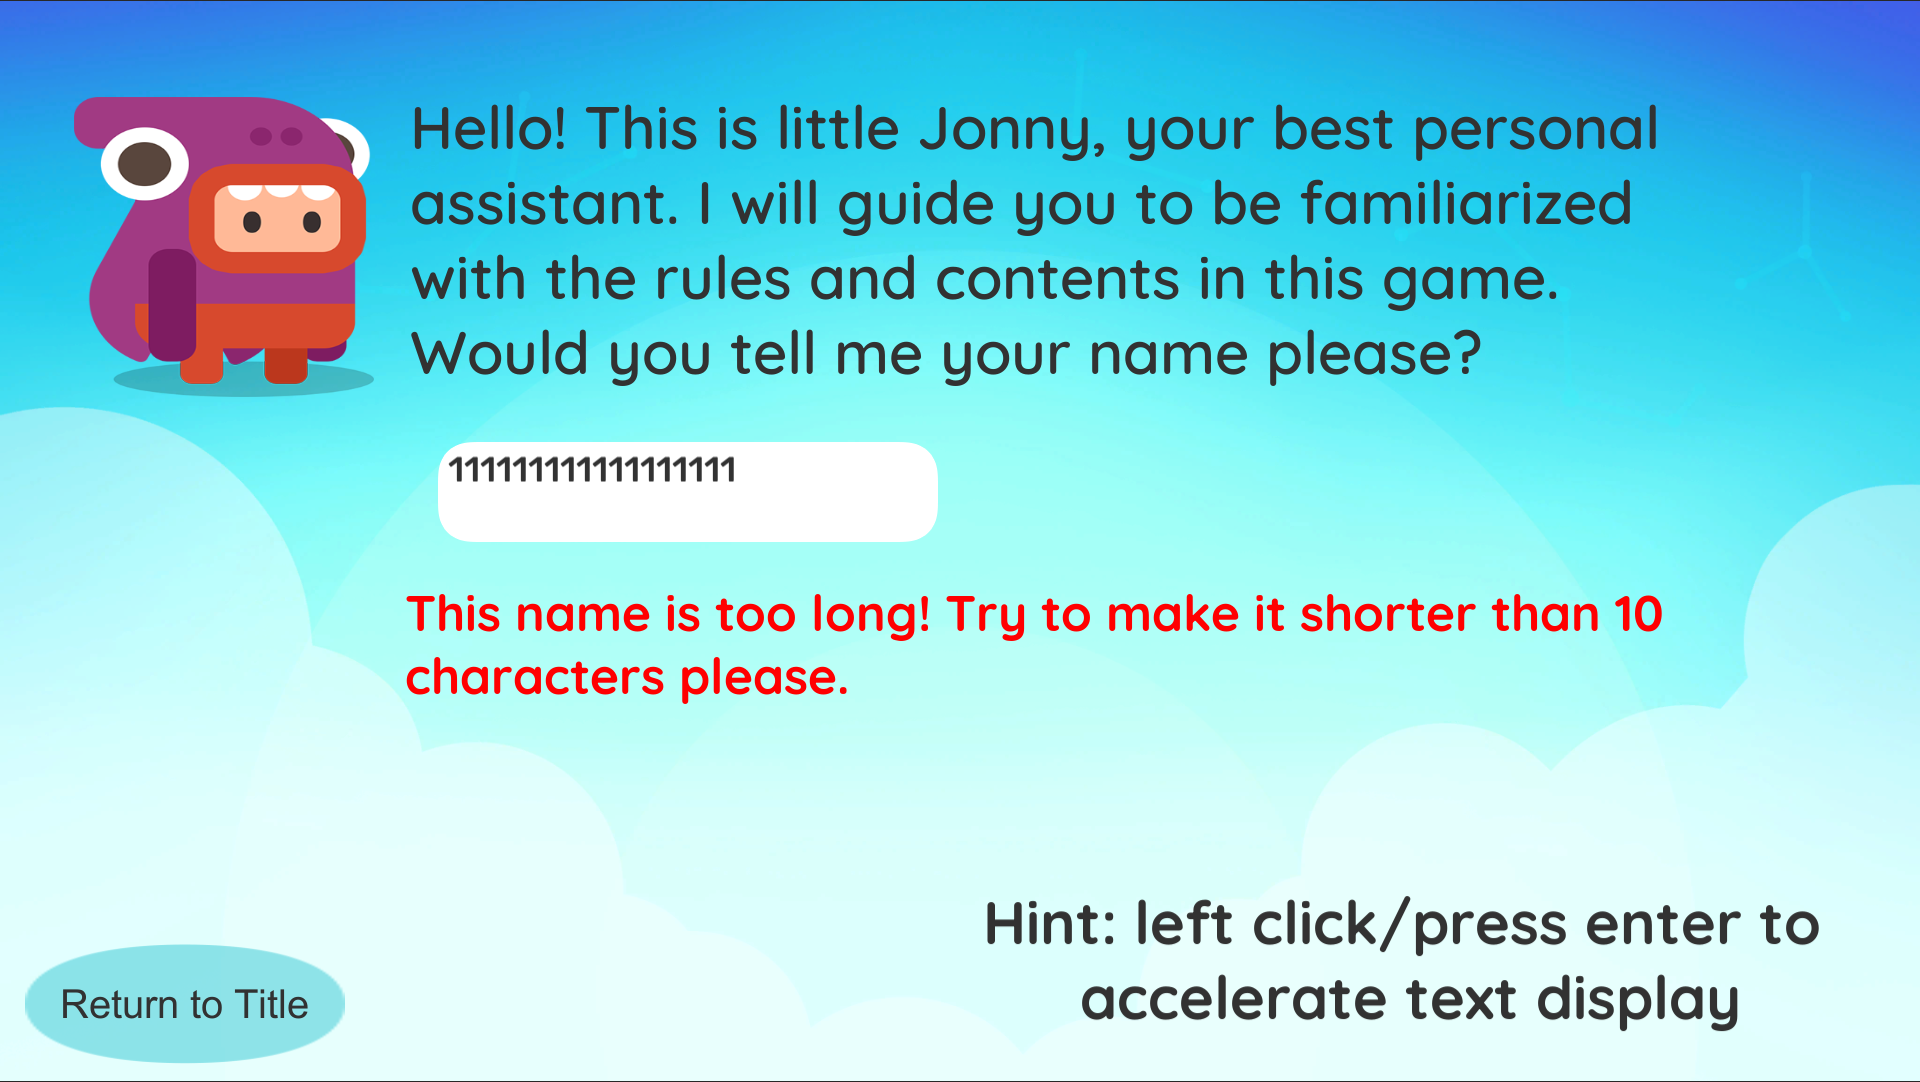
\includegraphics[width=1\textwidth]{Name_b.png}
\end{minipage}
}\hspace{-1pt}%在这里空一行会强制subfigure换行
\subfigure[name is repeated]{
\begin{minipage}[c]{0.48\textwidth}
\centering
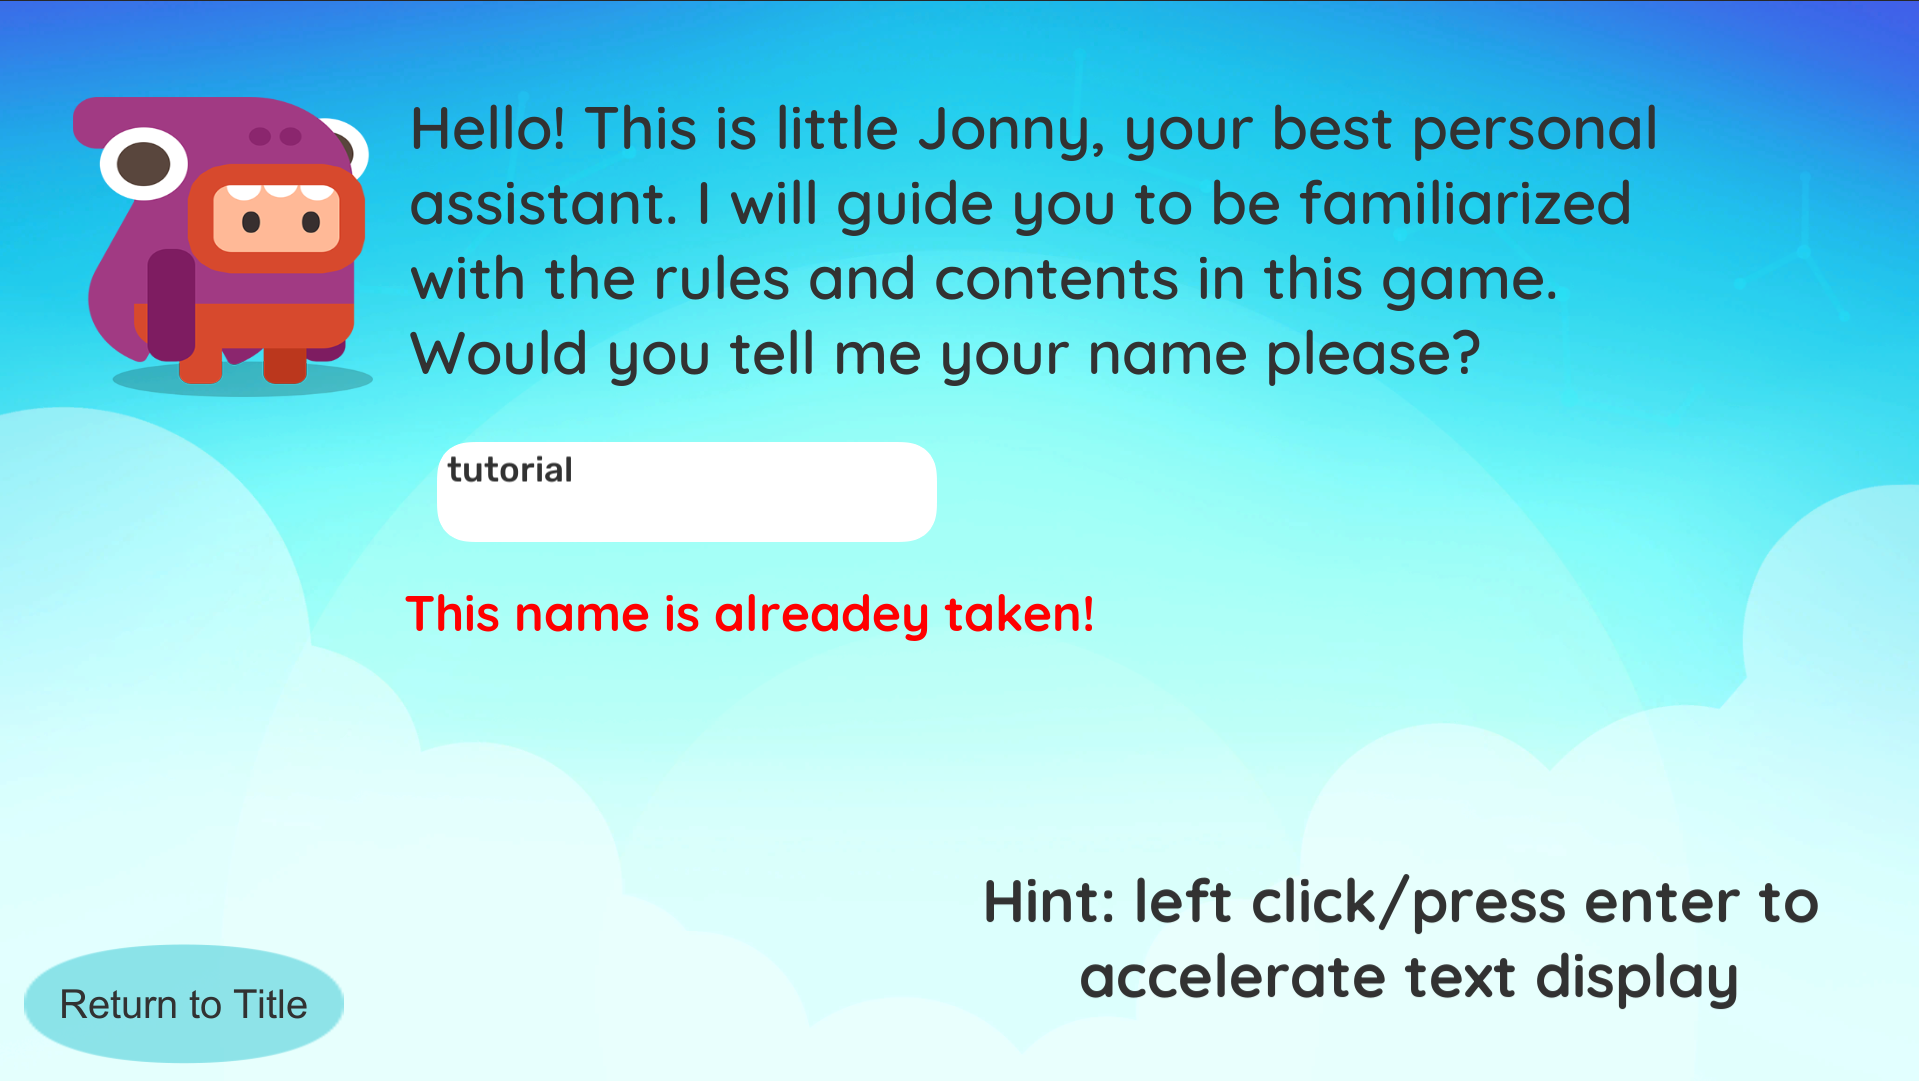
\includegraphics[width=1\textwidth]{Name_c.png}
\label{fig:name_c}
\end{minipage}
}\hspace{-1pt}%在这里空一行会强制subfigure换行
\caption{Introductory page: name input}
\label{fig:name}
\end{figure}

If the player inputs a valid username, a save file will be created automatically with some initialized data, and then the save file will be stored in the database. Players are initially given 15,000 points and two chances of tips for pop-up quizzes. They could get more points by playing the mini-game and use points to buy more chances of tips or other useful tools in the shop. Additionally, It is worth noting that there is a dialogue box on the bottom right of the introductory page, which tells players how to accelerate text display. We have made an animation that displays text character by character rather than showing everything at once. Players could control the display speed by left clicking or pressing the enter key. This design aims to improve interactivity with players.

\subsection{Scenario-based privacy question}

The 75 scenarios for privacy questions constitute the central part of this game. We will use a storytelling tone to vividly illustrate each scenario to players rather than mechanically state the whole question. Otherwise, the game would be tedious and concatenated by dullness. We also use second-person narration to simulate the scenario so players would feel like they are in the story.  All the efforts on the narrative techniques aim to simulate a real life situation for players.

\begin{figure}
    \centering
    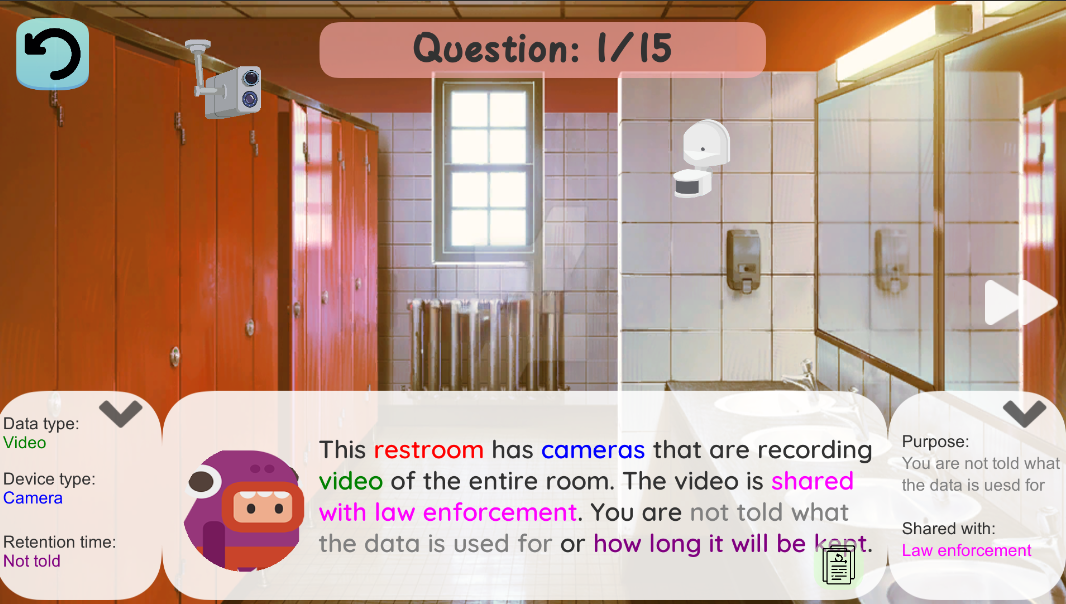
\includegraphics[width=0.8\textwidth]{Interface.png}
    \caption{Interface of privacy question: Public Restroom}
    \label{fig:interface}
\end{figure}

Figure \ref{fig:interface} shows an example scenario of the interface for privacy questions. The background is an image of the scene indicating the player's current location, which is the public restroom in this case. We use different colors to emphasize factors that may affect privacy preference, as shown in table \ref{tab:color}. By changing the colors, it would be helpful to present each scenario to players. Furthermore, not only using plain text, we also put some images of IoT devices in the background to illustrate the current type of device that collects privacy information. For example, there is a camera mounted on the ceiling and a presence sensor installed on the wall beside the restroom mirror. Another purpose of doing this is to imply to players the possible position where the IoT devices are installed in real life. Additionally, we added a reference list on both sides of the dialogue box so players could quickly check those factors on the privacy question.

\begin{table}[htbp]
    \begin{center}
    \begin{tabular}{ |c|c|c|c|c|c|c|}
        \hline
        \textbf{Factor} & Location & Device type & Data type & Retention & Shared & Purpose\\
        \hline
        \textbf{Color}& Red & Blue & Green & Purple & Magenta & Grey \\
        \hline
        \end{tabular} 
    \end{center}
    \caption{Different colors corresponding to different factors}
    \label{tab:color}
\end{table}

Players are asked two privacy questions about their comfort levels and decisions regarding the scenario mentioned before when all factors are presented. The interface for selecting comfort levels and decisions is shown in figure \ref{fig:select}. The system will record players' choices as soon as they make their selections and store them in the database. Consequently, they do not have to save their data manually due to this autosave feature.

\begin{figure}[htbp]
\center
\subfigure[comfort level]{
\begin{minipage}[c]{0.48\textwidth} %自行调整,太大的话会自动换行
\centering
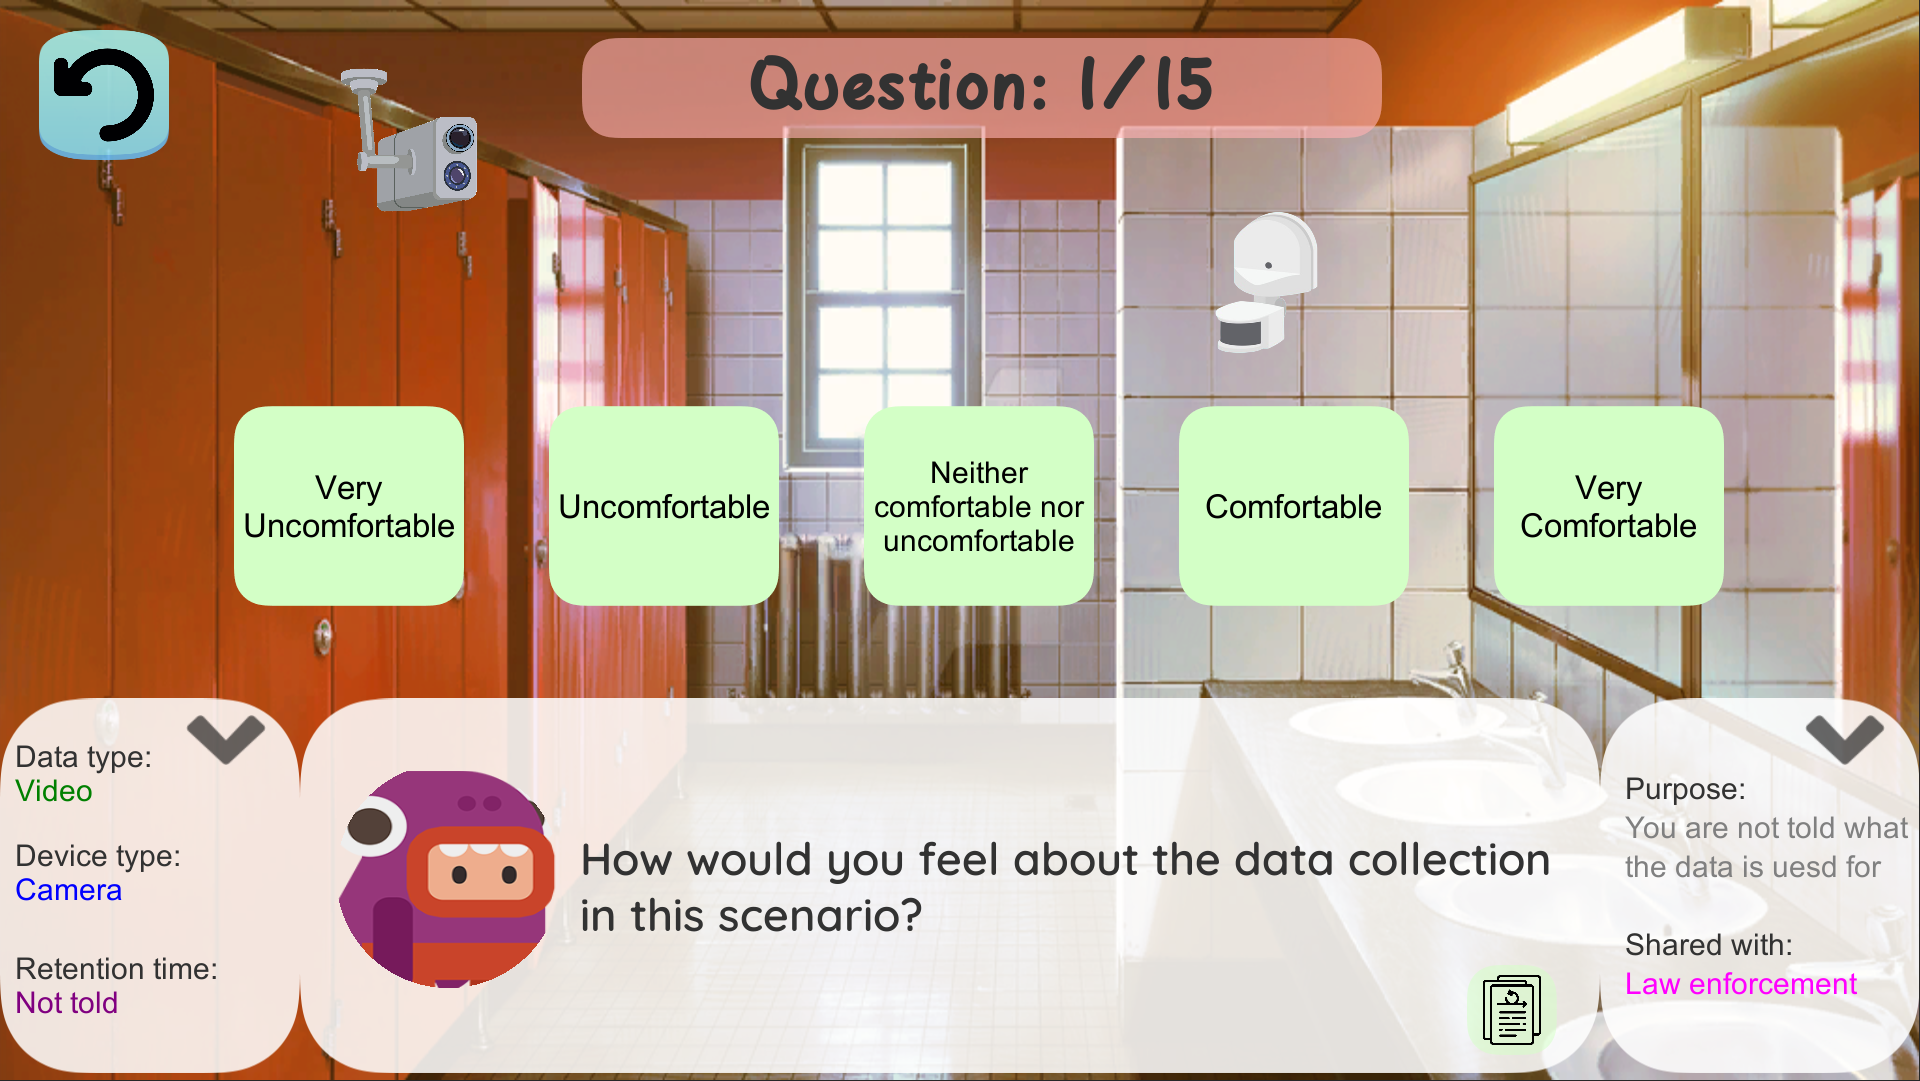
\includegraphics[width=1\textwidth]{Comfort.png}
%width相加大于1时自动换行
%自行调整width \vsapce \hspace
\end{minipage}
}\hspace{-1pt}%调整subfigure的间距
\subfigure[allow/deny decision]{
\begin{minipage}[c]{0.48\textwidth}
\centering
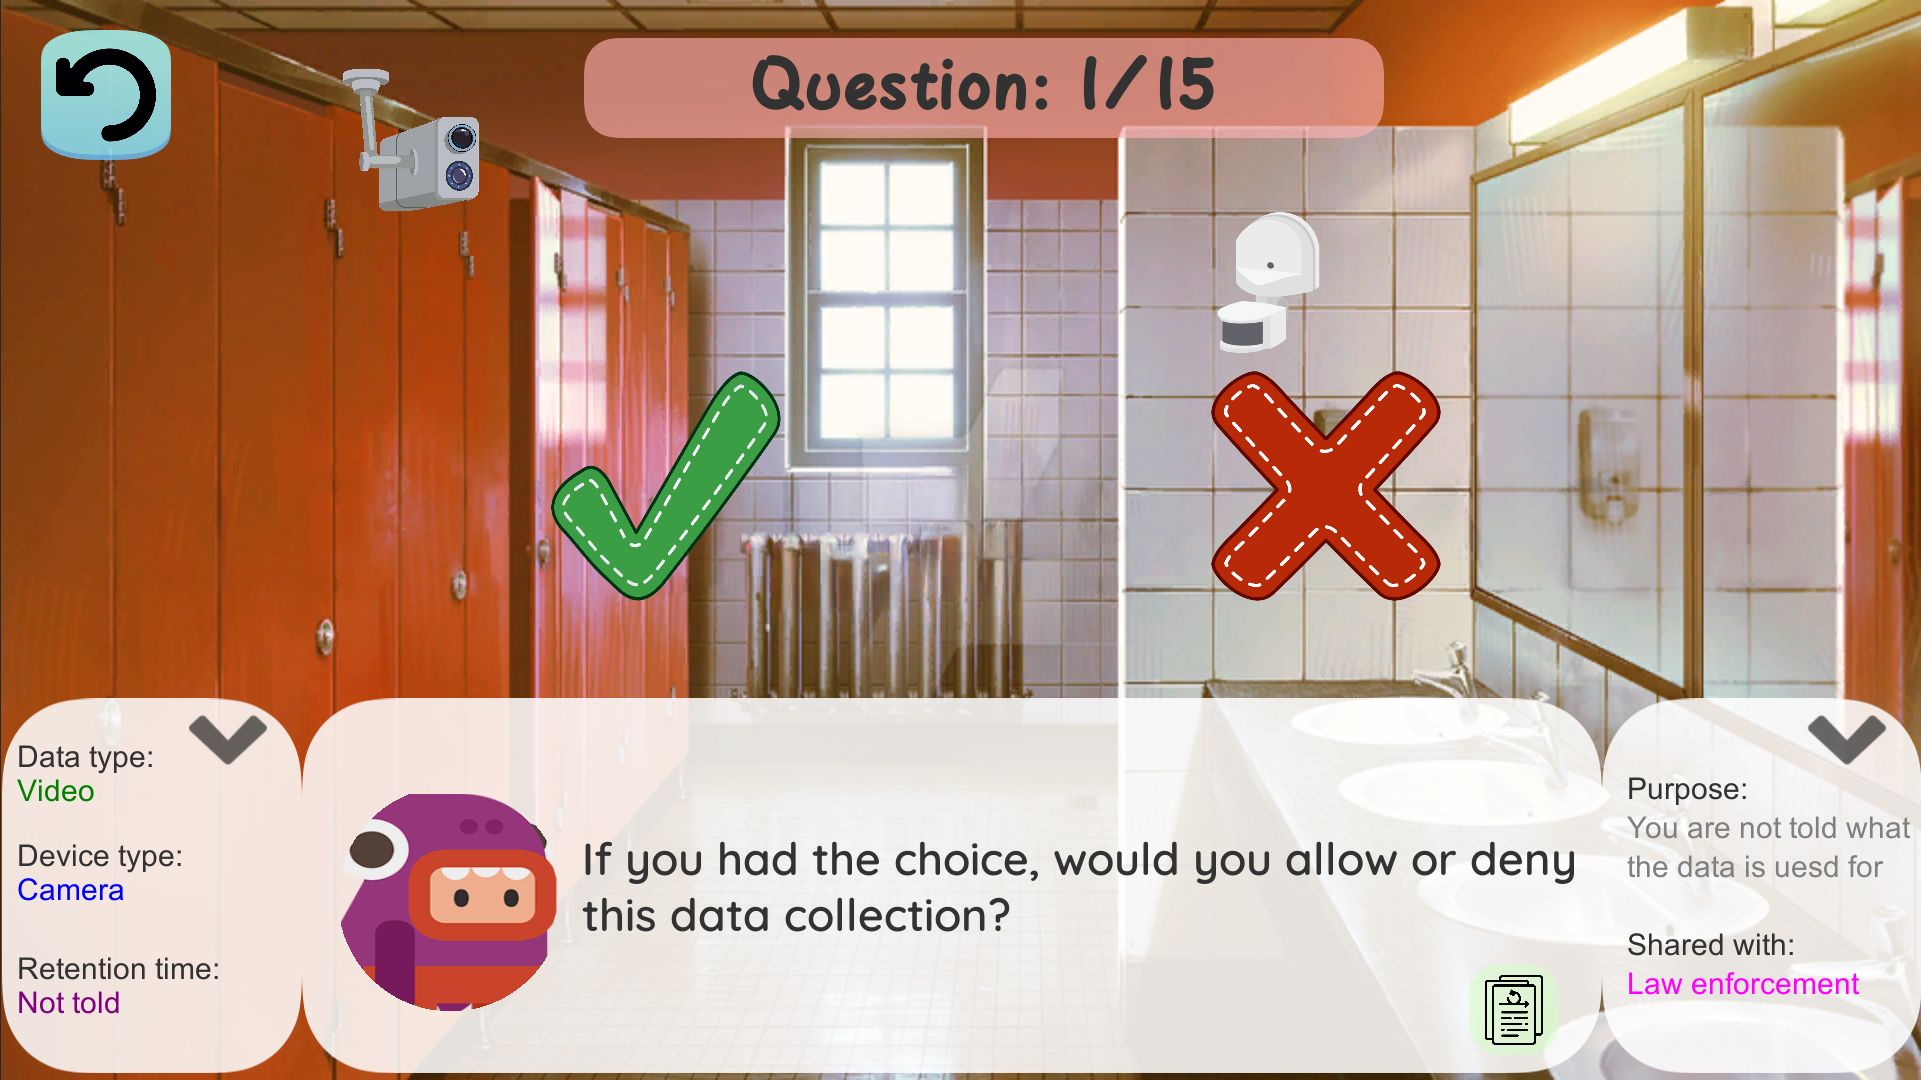
\includegraphics[width=1\textwidth]{Decision.png}
\end{minipage}
}\hspace{-1pt}%在这里空一行会强制subfigure换行
\caption{Interface of comfort level and allow/deny decision}
\label{fig:select}
\end{figure}

Another feature in the design of privacy questions is that we made each scenario consecutive, which means there is a relationship between two consecutive scenarios. For instance, a scenario would be a camera recording a video of the entire room in the public restroom, and the video will be shared with law enforcement. In this question, players are not told how long the data will be kept. Subsequently, we will keep every factor unchanged except for the retention time in the following scenario. Hence the next question would be how would they feel if players are told that the data will be kept for a certain amount of time, one year or until the purpose is satisfied. The reason behind this setting is that we considered that if every factor is changed, players would feel confused and could not make up their minds accordingly and resulting in a mess. The nuance of factors between two scenarios is helpful when analyzing the effect on individuals' privacy preferences.

\subsection{Pop-up quizzes and tips}
\label{section:quiz}
The pop-up quizzes usually appear before the privacy questions. The interface for pop-up quizzes is shown in figure \ref{fig:quiz}. Five icons, each representing one kind of IoT device, are located in the middle of the image. There will always be one correct answer, with the rest four icons randomly generated from the IoT device pool. A quiz tag resides on the top right corner of the interface, which indicates the current quiz ID and state. The quiz ID will be referenced on the quizzes' results page, which tells the player's performance on each quiz. Players could try the same quiz multiple times to improve their accuracy, and the number of tries will be recorded until they get correct. The quiz state will show whether players get the correct or wrong answer on that quiz, and show as none if it is the first time to attempt the quiz.

\begin{figure}
    \centering
    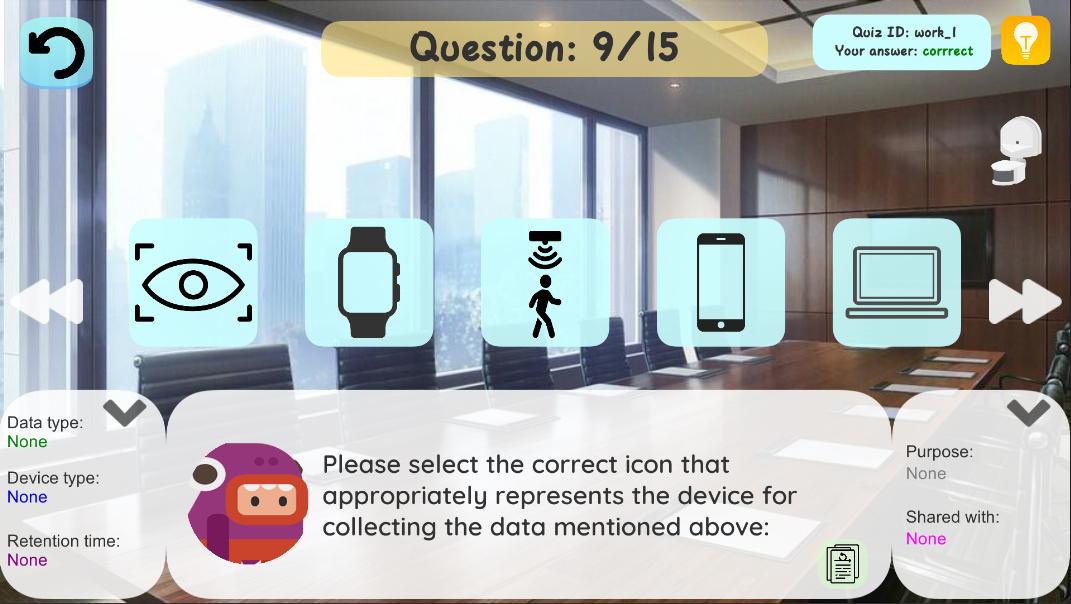
\includegraphics[width=0.8\textwidth]{Quiz.png}
    \caption{Interface of pop-up quizzes}
    \label{fig:quiz}
\end{figure} 

The tips icon on the right side of the quiz tag also appears along with the quiz. Players could consume one chance of tips to check the hints if they feel stuck on the quiz. There are two levels of tips. In the first level, we will hint to players by giving more information about the IoT device and providing some ideas to infer the correct answers. In the second level, we will directly tell players which icon is correct. The usage of tips will also be stored in the database to provide feedback about players' degree of knowledge on corresponding IoT devices. We also provide a shortcut to buy hints paying with points if players do not have one. The current number of chances and points will be presented if players decide to use hints.

\subsection{Log and jump-scene button}
\label{section:log and jump-scene}

Referring back to \ref{fig:quiz}, we could find a dialogue box in the top middle of the privacy question interface, which indicates the index of the current scenario over the total number of scenarios on this location. As mentioned in section \ref{section:main page}, a location icon includes a subset of scenarios whose privacy events happened in that location. The numbers of one subset of scenarios grouped by location are presented in table \ref{tab:factors} in the \textbf{Location} row. We could see that most locations have 15 scenarios except for \textit{home} and \textit{friend's home}, which are 7 and 8, respectively. We considered that 15 scenarios are too many for a single location, so we divided each location into several separate scenes, with each scene having 4 or 5 scenarios. When players finish the privacy questions in one scene, they can press the right arrow button to proceed to the next scene, which contains another 4 or 5 scenarios. A left arrow button also allows players to jump back to the previous scene. Furthermore, if players want to change their minds, instead of going through every scenario in normal order, they could use this jump-scene button to jump to different scenes quickly.

To make the scenario texts self-contained, we added a log function that records the texts in the dialogue box and the player's choices. The log icon locates in the bottom right corner of the dialogue box. If players forget the context of the scenario or their choices, they could review it by clicking the log icon and then a scroll view will show up. Figure \ref{fig:log} shows the log of players' comfort level, decision and answer to a pop-up quiz, respectively. The logs will be cleared if players quit the game, move to another location, or jump to another scene.

\begin{figure}[htbp]
\center
\subfigure[log of comfort level]{
\begin{minipage}[c]{0.48\textwidth} %自行调整,太大的话会自动换行
\centering
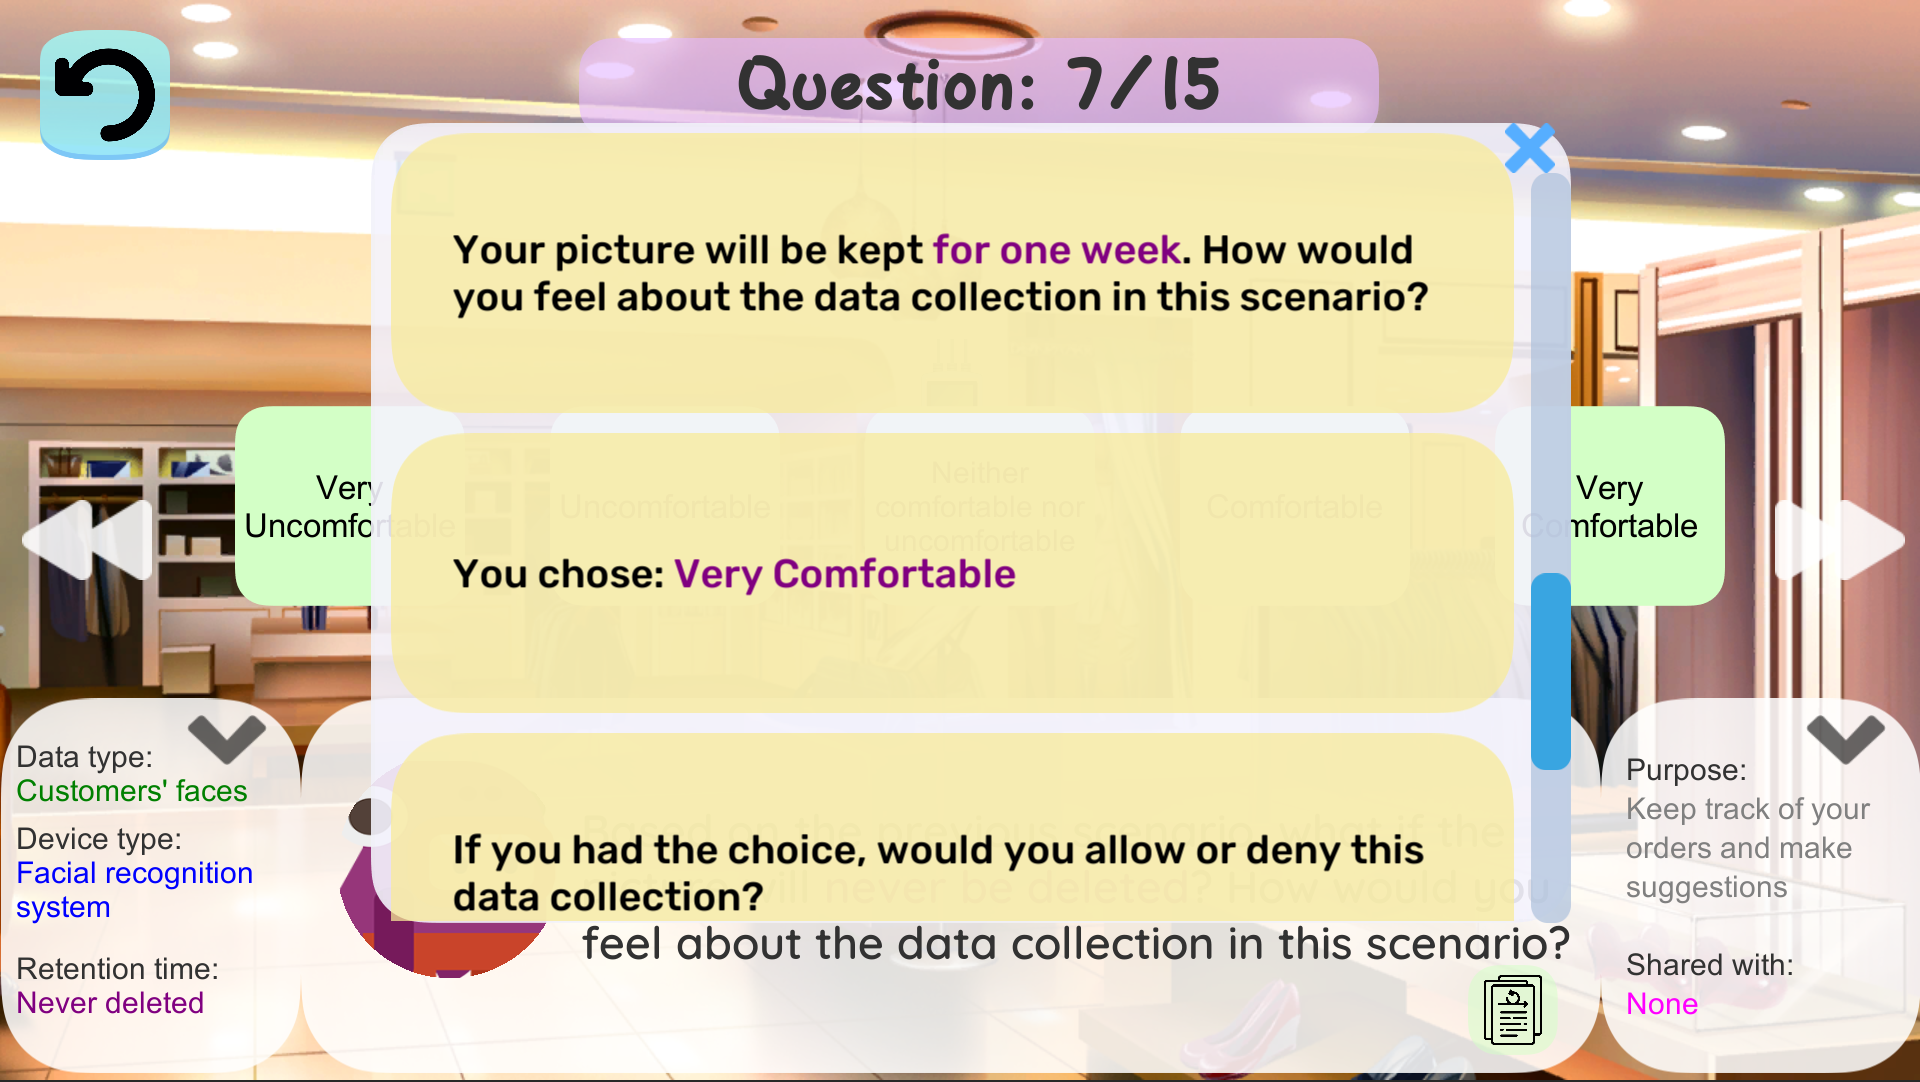
\includegraphics[width=1\textwidth]{Log_a.png}
%width相加大于1时自动换行
%自行调整width \vsapce \hspace
\end{minipage}
}\hspace{-1pt}%调整subfigure的间距
\subfigure[log of decision]{
\begin{minipage}[c]{0.48\textwidth}
\centering
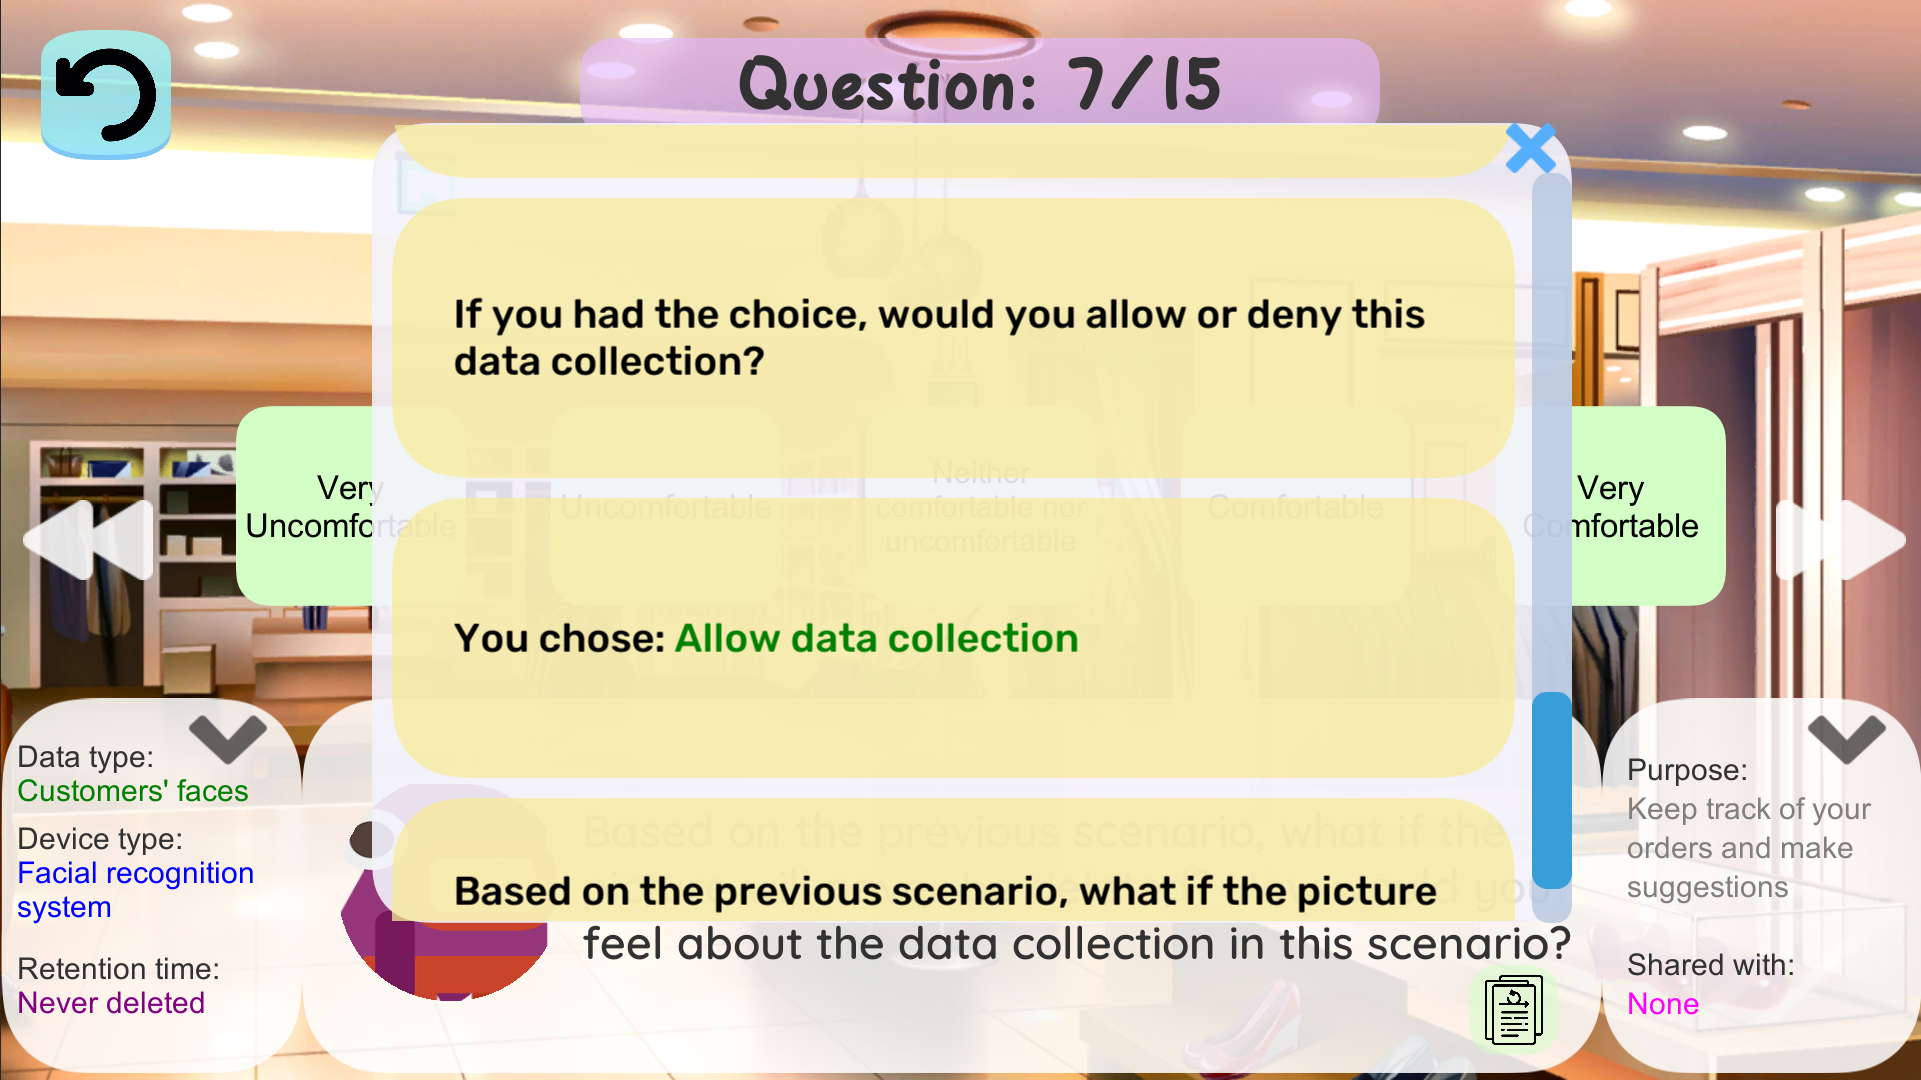
\includegraphics[width=1\textwidth]{Log_b.png}
\end{minipage}
}\hspace{-1pt}%在这里空一行会强制subfigure换行
\subfigure[log of pop-up quiz]{
\begin{minipage}[c]{0.48\textwidth}
\centering
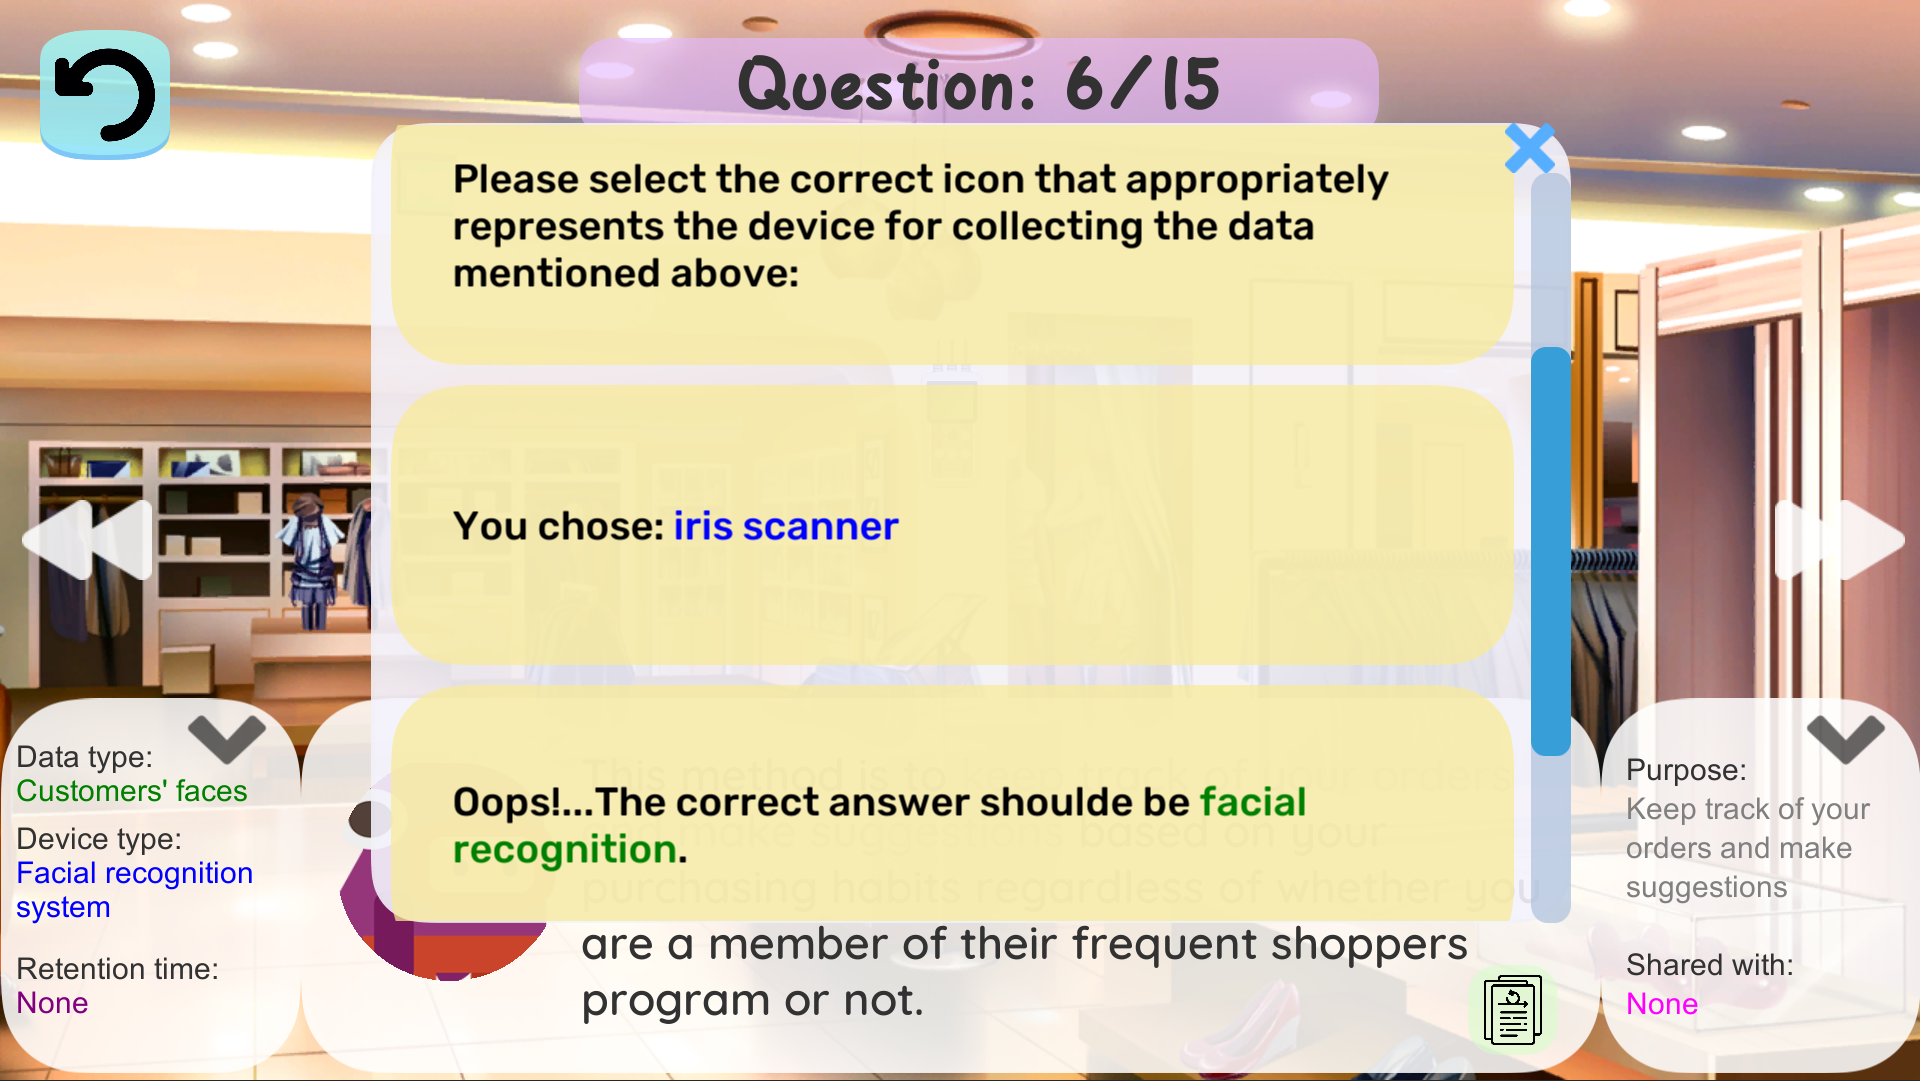
\includegraphics[width=1\textwidth]{Log_c.png}
\label{fig:log_c}
\end{minipage}
}\hspace{-1pt}%在这里空一行会强制subfigure换行
\caption{Logs for texts and player's choices}
\label{fig:log}
\end{figure}

\subsection{Mini-game and shop}
\label{section:mini-game}

In case players get bored when reading a large amount of text, we embedded a mini-game into this project. The name of this mini-game is \textbf{Happy Eliminating}, a great little game to pass the boring time. Due to its simple rule and unique playability, this game has been widely deployed on mobile devices, and we transferred it into our game. According to research about the playability of mobile games, in the evaluation of games, there are three essential modules: game usability, mobility, and gameplay \cite{Korhonen}. We believe that deploying the game \textbf{Happy Eliminating} on our project would help improve the playability of our game. 

The interface of the mini-game is shown in figure \ref{fig:game}. The players' current points are located in the top left corner, and the tutorials for the mini-game and other buttons reside in the top right corner. The game rule is simple, and players are easy to be addicted to it. There are nine rows and fifteen columns on the game board, with one of six different small blocks on each entry. The blocks are eliminated by putting more than three identical blocks in a line, horizontally or vertically, but these blocks must be adjacent. New blocks will be generated at the top to substitute the eliminated blocks. Players could drag the block to switch its position with its adjacent block. If the requirements to eliminate blocks are not met after switching, the block would return to its original position. There is a timer right below the game board. We set the timer to 120 seconds, and the game is over when the timer counts down to zero.

A toolbox on the right side of the game board contains three kinds of IoT devices. These devices have various functions and could be bought from the shop. The first one is the smartphone, whose function is temporarily increasing the number of points for successfully eliminating each one of the blocks. It has a charge gauge and was initially disabled while eliminating blocks each time would charge the device. The device is ready to use when fully charged and needs to recharge after use. The exact mechanism also applies to the second IoT device, a smartwatch. The function of the smartwatch is to freeze the timer for a while. Different from the previous two devices, the third one, the tablet, does not need to charge. It is more potent in that it could randomly destroy one row of blocks, instantly giving a large amount of points, but it needs to cool down for a while after used.

\begin{figure}
    \centering
    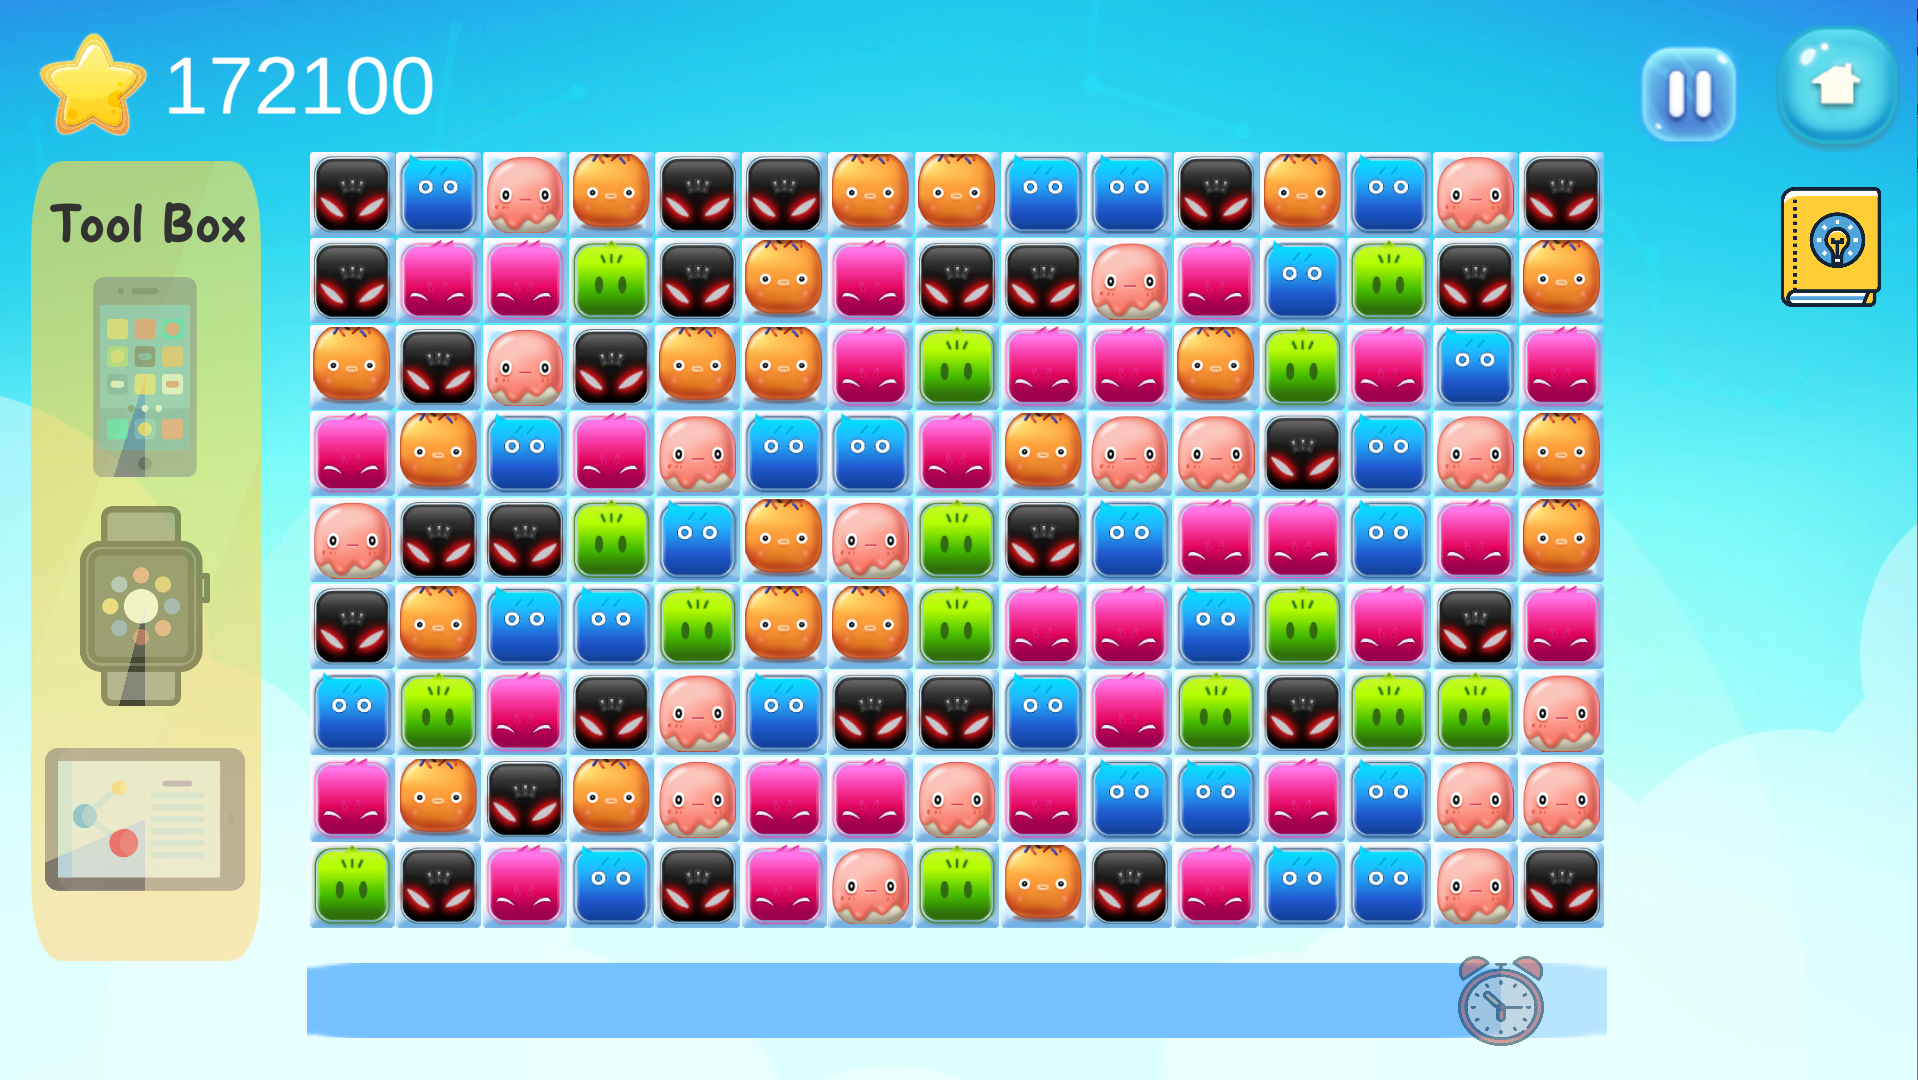
\includegraphics[width=0.8\textwidth]{Mini-game.png}
    \caption{Interface of mini-game: Happy Eliminating}
    \label{fig:game}
\end{figure}

\begin{figure}
    \centering
    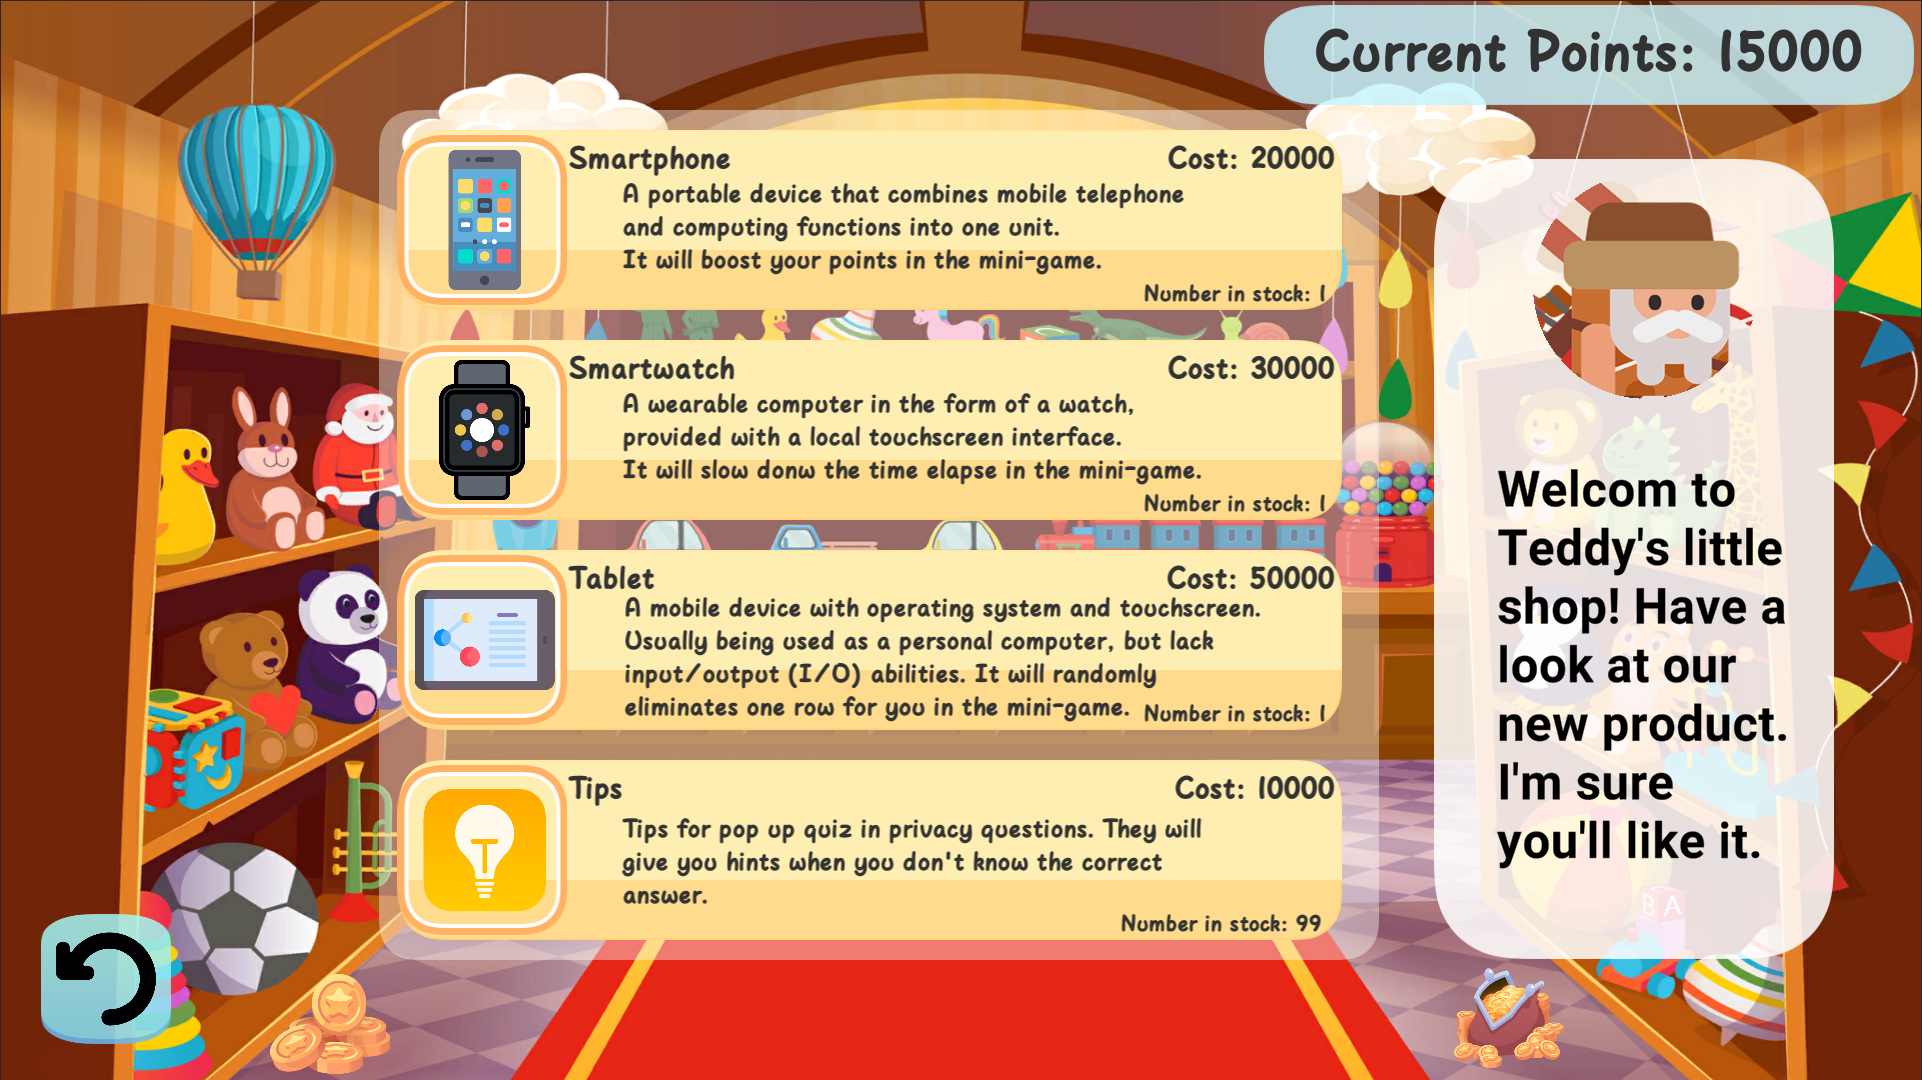
\includegraphics[width=0.8\textwidth]{Shop.png}
    \caption{Interface of the shop}
    \label{fig:shop}
\end{figure}

The tools described above are available in the shop, whose interface is shown in figure \ref{fig:shop}. Players could buy four items in the shop, three of which are IoT devices used in the mini-game, while the last item is tips for the pop-up quizzes. The points earned through the mini-game could be used to buy some IoT devices to get more points or buy tips to improve pop-up quizzes' accuracy. The cost for each item is located on the top right side of the product description. We would increase the cost of tips each time players buy one of them, which means it would be very costly if players bought too many tips. The costs for the other three items are fixed because there is only for each IoT device, there is only one left in stock.

\subsection{Results pages}

We divided the results pages into two parts. In the first part, we will present to players the most and the least factors that affect their privacy preferences. Additionally, we will use pie charts and bar charts from visualizing the six factors' correlation coefficients. Figure \ref{fig:visualze} is an example in the results pages of the visualization of factors that impact comfort level. Figure \ref{fig:pie} is a pie chart for the six factors shown in various colors. The merit of using the pie chart is that we could quickly understand the proportions for different factors at a glance. Factors with greater importance correspond to larger areas in the pie chart.

Figure \ref{fig:bar} is a bar chart for the six factors. The bar chart provides a good view of the exact values of factors' correlation coefficients. However, instead of taking the absolute value as we did in the pie chart, we kept the sign for the coefficients such that we could analyze the effect of factors both qualitative and quantitatively. Coefficients with positive signs represent that the corresponding factors have positive relationships between players' privacy preferences and vice versa. A positive relationship means that for a certain factor, based on the ranking criteria in table \ref{tab:factors}, the higher the rank, the higher possibility that players are comfortable with the data collection or are more likely to allow the data collection. For example, in figure \ref{fig:bar} the factor \textbf{Location} is green and has the longest bar length. We could conclude that factor \textbf{Location} has the greatest impact on the players' privacy preferences, and the more space confidentiality the location has, the more comfortable they would feel. A counterexample is \textbf{Retention time}, whose correlation coefficient is negative, meaning that the shorter the time data is retained, the more comfortable players would feel.

\begin{figure}[htbp]
\center
\subfigure[pie chartl]{
\label{fig:pie}
\begin{minipage}[c]{0.48\textwidth} %自行调整,太大的话会自动换行
\centering
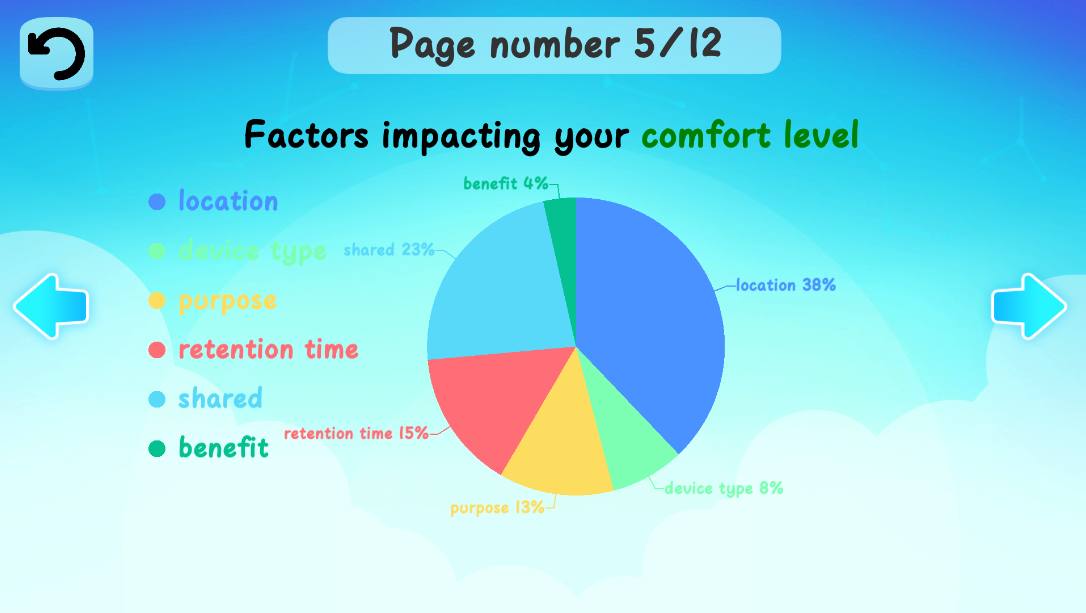
\includegraphics[width=1\textwidth]{Pie.png}
%width相加大于1时自动换行
%自行调整width \vsapce \hspace
\end{minipage}
}\hspace{-1pt}%调整subfigure的间距
\subfigure[bar chart]{
\label{fig:bar}
\begin{minipage}[c]{0.48\textwidth}
\centering
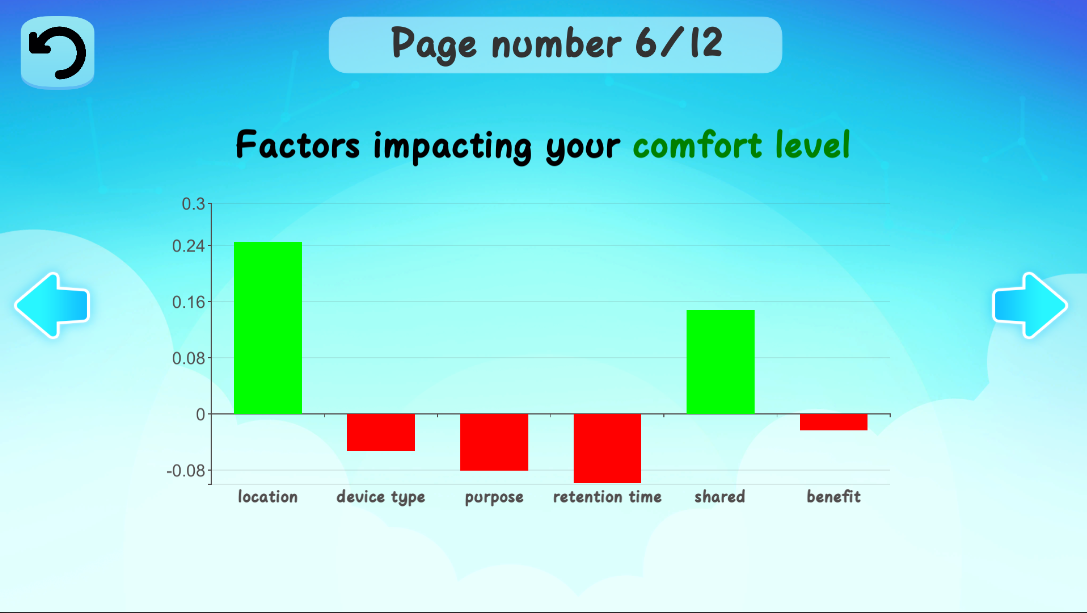
\includegraphics[width=1\textwidth]{Bar.png}
\end{minipage}
}\hspace{-1pt}%在这里空一行会强制subfigure换行
\caption{Visualize factors that impact comfort level}
\label{fig:visualze}
\end{figure}

In the second part, we will provide feedback on pop-up quizzes, as shown in figure \ref{fig:performance&tips}. We will evaluate how players are familiar with the IoT devices based on their correctness on related devices, as shown in figure \ref{fig:performance}. The usage of tips will also be presented in figure \ref{fig:tips}.

\begin{figure}[htbp]
\center
\subfigure[performance]{
\label{fig:performance}
\begin{minipage}[c]{0.48\textwidth} %自行调整,太大的话会自动换行
\centering
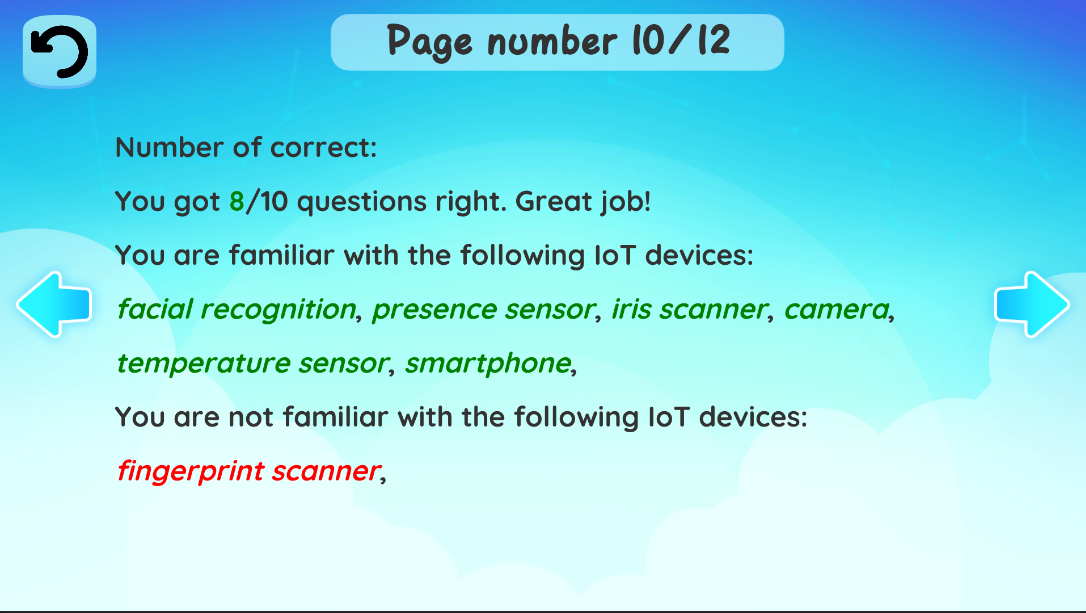
\includegraphics[width=1\textwidth]{Performance.png}
%width相加大于1时自动换行
%自行调整width \vsapce \hspace
\end{minipage}
}\hspace{-1pt}%调整subfigure的间距
\subfigure[tip states]{
\label{fig:tips}
\begin{minipage}[c]{0.48\textwidth}
\centering
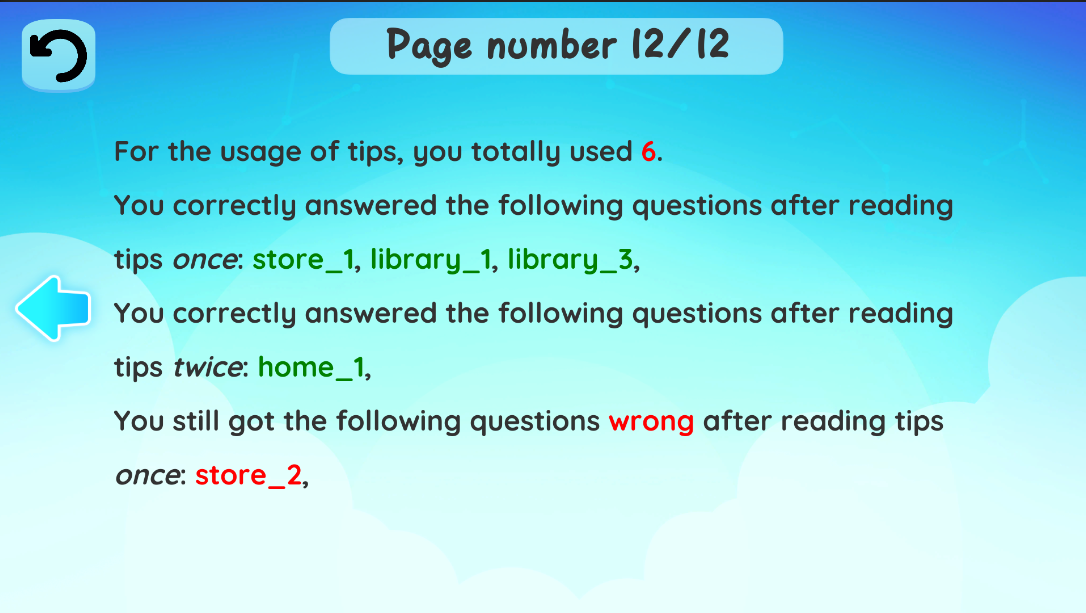
\includegraphics[width=1\textwidth]{Tips.png}
\end{minipage}
}\hspace{-1pt}%在这里空一行会强制subfigure换行
\caption{Players' performances on pop-up quizzes and tips states}
\label{fig:performance&tips}
\end{figure}

\chapter{Game Implementation}

In this chapter, we will introduce the detailed process of implementing the game, including the interfaces, button controller and statistical models. We will also discuss some techniques we used with Unity and C\# scripts.

\section{UGUI}

Unity Graphical User Interface (UGUI) is a UI toolkit for developing user interfaces for games and applications provided by Unity in the version above 4.6. It is based on the UI system of GameObject, the base class for all entities in Unity scenes, to arrange and style user interfaces. It provides a functional event system module with various classes for mouse clicking, pointer moving, item dragging, and keyboard inputting. UGUI is widely used in this project to perform various functions, including interfaces, button controllers, and background.

\subsection{Interface layouts}
\label{section:interface}

In the first step of implementation, we need to lay out the interfaces for every game scene. We bought a GUI kit from the internet containing game materials such as buttons, frames, icons, and fonts. Since UGUI uses GameObject-based UI system, we need to create a GameObject for each interface and adjust the corresponding parameters properly. 

Figure \ref{fig:UGUI} shows the inspection panel of a UGUI GameObject. It has three components: Rect Transform, Canvas Renderer, and Image. Almost every UGUI GameObject has the first two components, while the third component depends on the attribute of the UGUI. For example, if we want to add a background to the scene, we need to set its source image in the Image component. On the other hand, if we want to add text to the dialogue box, it is apparent that we do not need a source image for text. Instead, we need a Text component that contains the plain texts we want to show in the dialogue box and other information such as the font size or the color of the text. The first component, Rect Transform, is the most crucial part of the UGUI because it controls the layout of interfaces. It could modify the interface's coordinate, size, anchors, pivot, and relative scale. In this example, the parameters in figure \ref{fig:UGUI} are used for the background, whose coordinate is set on original (0,0,0) and size is set to $1920\times1080$, which is the resolution of our game. We repeated the same procedure for all interfaces.

\begin{figure}
    \centering
    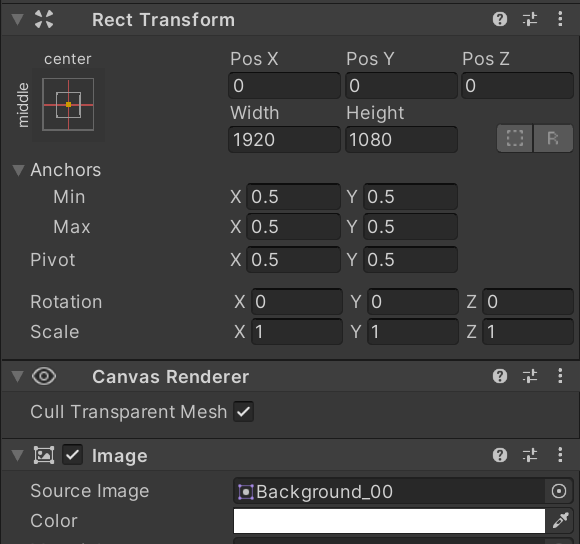
\includegraphics[width=0.65\textwidth]{UGUI.png}
    \caption{UGUI components}
    \label{fig:UGUI}
\end{figure}

\subsection{Button controllers}

Aside from the three components introduced in the previous section, there is another vital component in UGUI: Button. The Button component incorporates an event system trigger that handles the event when triggered by a pointer or keyboard. We added an \texttt{OnClick} event for every button such that all buttons could perform their duties. There are two ways to add \texttt{OnClick} event. The first one is directly adding events in the Button component, as shown in figure \ref{fig:OnClick}, which is an example of the Button component for \textbf{New Game} button on the start page. We could see two clicking events attached to the \textbf{New Game} button. The first one calls the \texttt{LoadScene2()} method in the \texttt{SceneManager} class, as indicated in the dropdown window. The function will load a game scene specified by an index. The second event is an audio player. It calls the \texttt{Play()} method in the \texttt{AudioSource} class, which plays a sound effect when the button is clicked.

\begin{figure}[htbp]
\center
\subfigure[OnClick events in Button component]{
\begin{minipage}[c]{0.9\textwidth} %自行调整,太大的话会自动换行
\centering
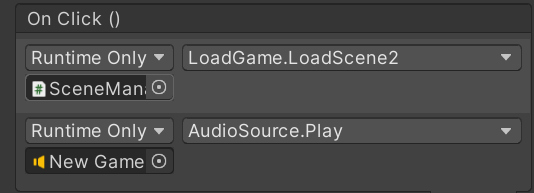
\includegraphics[width=0.8\textwidth]{OnClick.png}
%width相加大于1时自动换行
%自行调整width \vsapce \hspace
\end{minipage}
}\hspace{-1pt}%调整subfigure的间距
\subfigure[New Game button in the start page]{
\begin{minipage}[c]{0.9\textwidth}
\centering

\includegraphics[width=0.8\textwidth]{NewGame button.png}
\end{minipage}
}\hspace{-1pt}%在这里空一行会强制subfigure换行
\caption{OnClick events in \textbf{New Game} button}
\label{fig:OnClick}
\end{figure}

Even though the \texttt{OnClick} events are easily deployed in the Button component, it also has some drawbacks. One of the main drawbacks is repeatability. Since button controllers are widely used in this game, setting events for every button controller would be tedious. Hence we use the other way to deploy \texttt{OnClick} events, the C\# scripts. Unity has provided a class \texttt{IPointerClickHandler} which allows to set \texttt{OnClick} events with C\# scripts. Based on the concept of Object Oriented Programming (OOP), we encapsulated a class \texttt{MyButton} inherited from the \texttt{Button} class which defines all basic events for buttons. The function prototypes are shown in listing \ref{lst:MyButton}.


\begin{lstlisting}[caption={MyButton class},label={lst:MyButton},language=C++]
Using Unity.UI
public class MyButton : Button
{
    public override void OnPointerDown(PointerEventData eventData);
    public override void OnPointerUp(PointerEventData eventData);
    public override void OnPointerEnter(PointerEventData eventData);
    public override void OnPointerExit(PointerEventData eventData);
}
\end{lstlisting}

The class \texttt{Button} is included in the namespace \texttt{Unity.UI} which defines every type of UGUI. By inheriting the \texttt{Button} class, we have all events for buttons. Furthermore, we redefined four events inherited from the \texttt{Button} class using the \texttt{override} keyword. The function prototypes in lines 4 to 7 represent events for the following time: when the pointer is pressed, released, moved onto the UI, or moved out from the UI. 

Except for the most commonly used buttons, such as the \textbf{New Game} in figure \ref{fig:OnClick}, there are also some special buttons that have their specific duties. For instance, for those icon buttons such as department store and library shown in figure \ref{fig:main}, if players move a pointer onto the button, the size of the corresponding icon would be scaled by a factor of 1.2. As we did in the \texttt{MyButton} class, we encapsulated another class named \texttt{GeneralIconButton} for those icon buttons. We redefined the related events by overriding the methods inherited from its parents.

\begin{lstlisting}[caption={Different child class inherited from \texttt{Button} },label={lst:OtherButton},language=C++]
public class GeneralIconButton : MyButton
public class JumpSceneBtn : GeneralIconButton
public class ReturnStageBtn : MyButton, IPointerClickHandler
\end{lstlisting}

Listing \ref{lst:OtherButton} shows a list of child classes inherited from \texttt{Button}. Besides the first class introduced above, there are two more types of child classes: \texttt{JumpSceneBtn} inherited from \texttt{GeneralIconButton}, which provides the jumping scene function introduced in section \ref{section:log and jump-scene}. \texttt{ReturnStageBtn} inherited from \texttt{MyButton}, which has an \texttt{OnClick} event transferring players to the main page from every other scene of the game.

\subsection{DOTween}

DOTween is a powerful object-oriented animation engine for Unity. In this project, we use DOTween to make animations of UGUI, especially for UGUI transfer. In the interface of privacy questions shown in figure \ref{fig:interface}, we added two buttons that allow the reference list on both sides of the dialogue box to gradually move up and down if players want to hide it. The static method \texttt{DOLocalMove()} will be called by the transform of a GameObject to change its position gradually.

\begin{lstlisting}[caption={DOTween sequence},label={lst:DOTween},language=C++]
void myCallback();
Sequence seq = DOTween.Sequence();
seq.AppendInterval(1.3f);
seq.AppendCallback(myCallback);
\end{lstlisting}

We also used DOTween to delay function calls. The codes in listing \ref{lst:DOTween} show a way to use DOTween. Firstly, a \texttt{Sequence} object will be constructed. Then the method \texttt{AppendInterval()} will be called, with a float number as input. This method will tell the sequence how long it has to wait. The code in line 3 tells the sequence to wait for 1.3 seconds. The last step is to append the callback function, defined in \texttt{myCallback()}, to the sequence so that the callback function would be called after a waiting time. This technique is frequently used in the implementation of mini-game.

\section{Main Content Implementation}

The hierarchy panel on the left side of figure \ref{fig:Scene} shows all scenes built in this game, including an introductory page, a main page, a shop, a result page, a mini-game, two tutorials, and six locations for different scenarios of privacy questions and pop-up quizzes. In this section, we will introduce the implementation of the main content of this game. Specifically, we will introduce the detailed implementation procedures of the privacy questions and pop-up quizzes, mini-game, as well as the preference analysis models and performance feedback pages.

\begin{figure}[htbp]
    \centering
    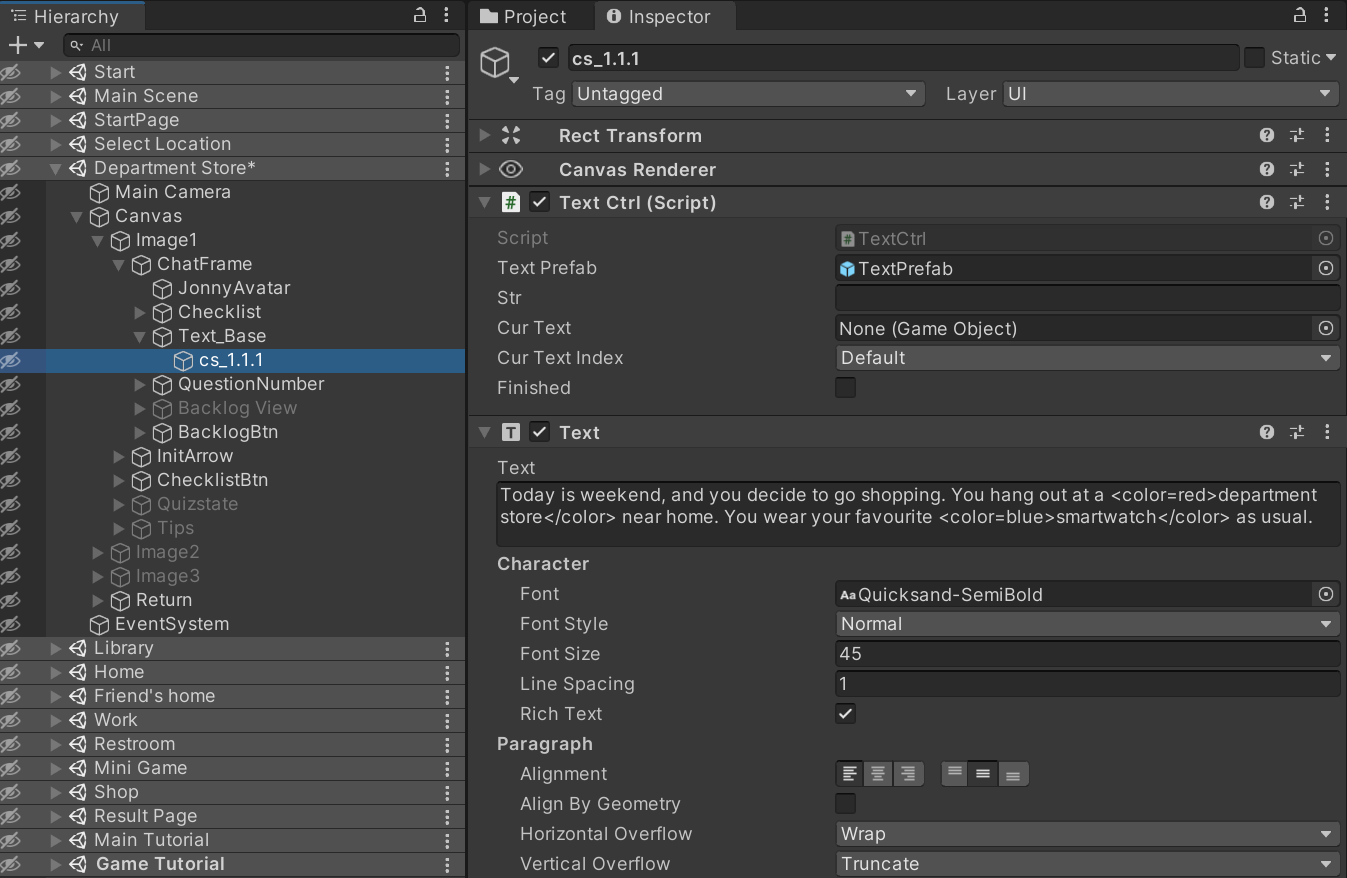
\includegraphics[width=0.8\textwidth]{Scene.png}
    \caption{Game scenes and inspection panel for texts of privacy questions}
    \label{fig:Scene}
\end{figure}

\subsection{Scenarios setup}

The assets we set for each scenario are also in the hierarchy panel in figure \ref{fig:Scene}, which illustrates a half-expanded hierarchy of GameObjects in the department store scene. The three roots in the hierarchy from top to down are Main Camera, Canvas, and EventSystem. The Main Camera is a device through which the players view the world. Players would not see anything without it. The Canvas is the parent of every UGUI GameObject, without which players would not see any UGUI GameObject. The third one is EventSystem, an empty GameObject with a C\# scripts for triggering events. Without it, all the system events, including button controls and keyboard inputs, would be invalid.

We put three images under the Canvas root to simulate three different scenes. Each image has its own child GameObjects, such as the dialogue box, jumping scene buttons, and a reference list. We use the dialogue box to communicate with players, telling them the setup of each scenario and asking them privacy questions. The right side of figure \ref{fig:Scene} is an inspection panel of the dialogue box. The inspection panel shows all components that attached to the GameObject of dialogue box. Except for the two compulsory components for UGUI described in section \ref{section:interface}, we also added a Text component for displaying texts and a \texttt{TextCtrl} class written in C\# scripts for controlling texts. The \texttt{TextCtrl} class would firstly load a GameObject prefab from the resources folder. A GameObject Prefab in Unity could be used as a template to create new Prefab instances in the scene. The loaded \texttt{TextPrefab} has already well-defined the parameters in the Rect Transform component; hence, we do not have to adjust the parameters manually. Furthermore, the \texttt{TextCtrl} controls the behaviors of text GameObject, such as the display speed of text and the order of text display. We defined all texts in a string array encapsulated in a static class \texttt{MainTextContent}. The \texttt{TextCtrl} will read the texts that will be displayed in the dialogue box by indexing the string array in \texttt{MainTextContent}.

\subsection{Player's information}
\label{section:player}

We created a class \texttt{Player} that stores player's information in games. Some of the essential fields in \texttt{Player} are defined in listing \ref{lst:player}. Codes in lines 3 and 4 are variables for username and current points. Using generic programming skills, we could create a list of variables with any types in the generic interface \texttt{List}. The attribute \texttt{tipStates} is a list of \texttt{TipState} instances, which are class objects that record the state of tips, including the number of used tips and the corresponding quiz ID for which players have used tips. Similar to \texttt{tipStates}, the attribute \texttt{quizstates} is a list of \texttt{QuizState} instances. The class \texttt{QuizState} has four attributes: two string variables for the current quiz ID and the correct answer to that quiz, an integer for the number of tries players did on that quiz, and a boolean indicating whether players answered correct or not on that quiz. The attribute \texttt{answers} is a list of \texttt{PrivacyQuestion} instances, and each instance records players' choices for privacy questions. The \texttt{PrivacyQuestion} class has three attributes: a string variable for the current scenario ID and two double variables for comfort level and decision corresponding to that scenario. The static method \texttt{Init()} is used to initialize variables in \texttt{Player}.

\begin{lstlisting}[caption={\texttt{Player} class fields },label={lst:player},language=C++]
public class Player
{
    // attribute
    static public string userName;
    static public float points;
    static public List<TipState> tipStates;
    static public List<QuizState> quizStates;
    static public List<PrivacyQuestion> answers;
    // method
    static public void Init();
}
\end{lstlisting}

When players make their choices of comfort levels and decisions, we need to update the information in the class \texttt{Player}. The information is updated as soon as players click the buttons for comfort levels and decisions, illustrated in figure \ref{fig:select}. Those buttons are attached with a \texttt{GeneralIconButton} component inherited from \texttt{MyButton}. Although they have some basic \texttt{OnClick} events, we also need to add a callback function that updates the player's information. Fortunately, the \texttt{Button} class has provided a method to dynamically add callback functions by calling \texttt{onClick.AddListener()}. The argument for \texttt{AddListener()} could be a function pointer or lambda expression.

Figure \ref{fig:callback} shows an example of how we add a callback function to the "Allow" button for the decision on data collection. Firstly, we use \texttt{Find()} function to search the scenario ID that corresponds to the privacy question and set the decision to 1 for allowing and 0 for denying the data collection. After updating the information, we will save the data immediately by calling the method \texttt{SaveByJSON()}. Then we will push the text that tells players what choice they have made into the log. Subsequently, we will use the index of the current text in the dialogue box to instantiate the GameObject for the subsequent text in the string array in \texttt{MainTextContent} and finally destroy the current GameObject.

\begin{figure}[htbp]
    \centering
    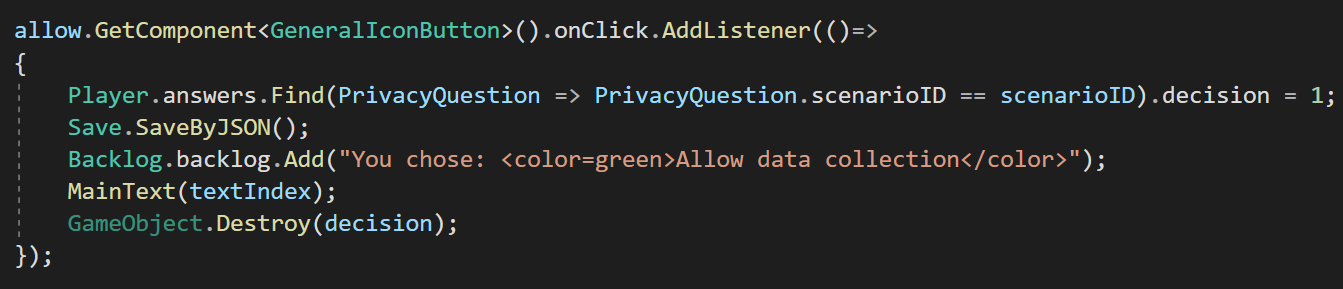
\includegraphics[width=0.9\textwidth]{Listener.png}
    \caption{Callback function for "allow" button}
    \label{fig:callback}
\end{figure}

We will repeat the whole process mentioned above in the section on pop-up quizzes. The callback function for updating the information about players' answers for the quizzes and the state of used tips will be implemented in the icon buttons for IoT devices in figure \ref{fig:quiz}. We designed an algorithm to randomly sample the IoT devices from the device pool without replacement. The detailed implementation method for the random sampling algorithm uses two arrays, one representing the sampled devices and the other representing the index of devices yet to be sampled. We will add a callback function for the icon button of each sampled device.

\subsection{Save game files}

There are multiple ways to store players' information about their game progress. The simplest method is to use serialized field, yet it could only keep some simple variables such as integers, and it does not support complicated data structures. Hence we decided to use JSON files to save the game data. Figure \ref{fig:Save/Load} shows two static methods for saving and loading data, encapsulated into a class \texttt{Save}. In \texttt{SaveByJson()}, we firstly create a \texttt{playerinfo} instance, which contains all the player's information mentioned in section \ref{section:player}. Then we call \texttt{JsonUtility.ToJson()} to convert player's information to JSON strings. In the following codes, a save file directory will be created if the directory does not exist, and then a stream writer object will be created for the system I/O. The last step is to write JSON strings to the stream writer and finally close the stream writer.

The procedure in function \texttt{LoadByJson()} is pretty much the same as that in the function \texttt{SaveByJson()} but in the opposite direction. In these steps, we will load the stored JSON strings to \texttt{playerinfo} such that players' game progressions are restored. It is worth noting that the comparison search for usernames mentioned in section \ref{section:intro} was also implemented in the class \texttt{Save}. The procedure is similar to loading by JSON, in which we use a stream reader to get a list of players' data. Then we will do a string comparison with the usernames stored in the list.

\begin{figure}[htbp]
\center
\subfigure[SaveByJson]{
\begin{minipage}[c]{\textwidth} %自行调整,太大的话会自动换行
\centering
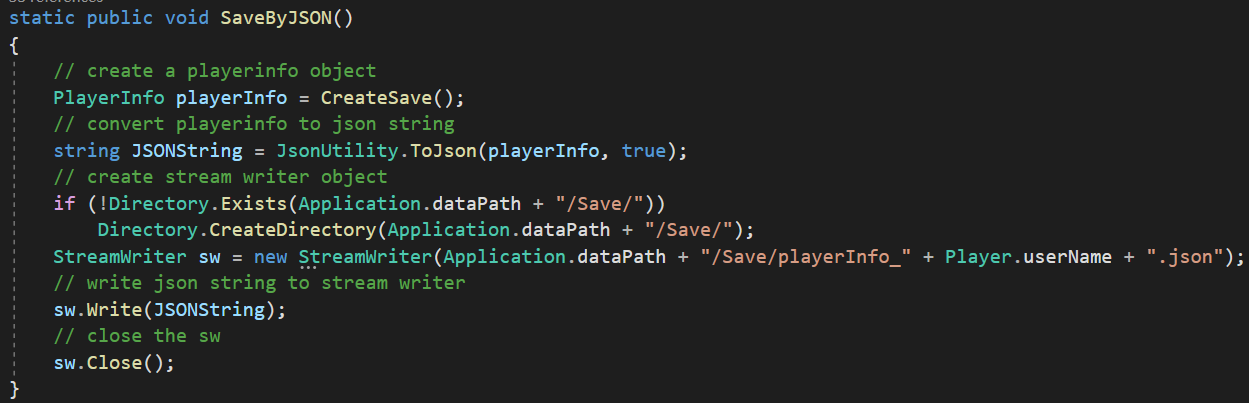
\includegraphics[width=0.9\textwidth]{Save.png}
%width相加大于1时自动换行
%自行调整width \vsapce \hspace
\end{minipage}
}\hspace{-1pt}%调整subfigure的间距
\subfigure[LoadByJson]{
\begin{minipage}[c]{\textwidth}
\centering
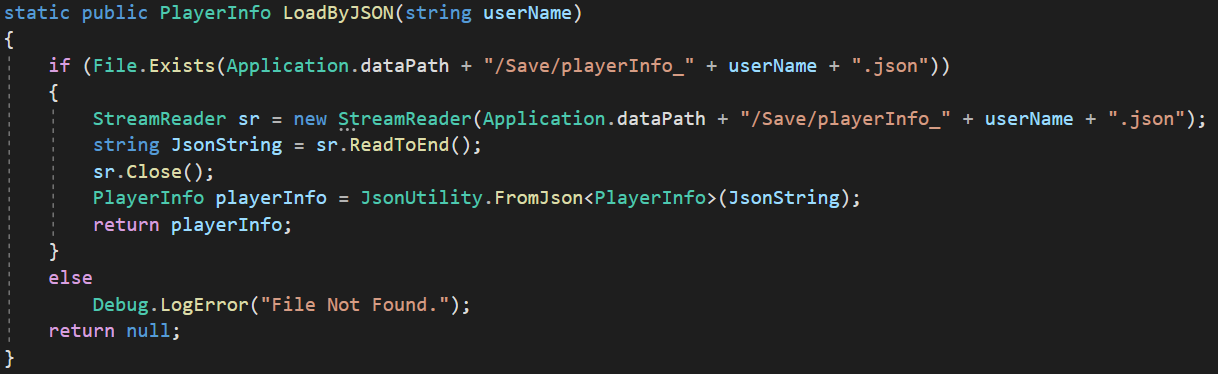
\includegraphics[width=0.9\textwidth]{Load.png}
\end{minipage}
}\hspace{-1pt}%在这里空一行会强制subfigure换行
\caption{Save and load functions}
\label{fig:Save/Load}
\end{figure}

\subsection{Statistical models and personalized feedback}

There will be two statistical models for individuals' privacy preferences, one for comfort levels and the other for decisions. The well-designed 75 scenarios are encoded into a \texttt{Dictionary} in class \texttt{ScenarioCode}. The codes in listing \ref{lst:scenario} illustrate the declaration of the variable \texttt{scenarios} and an example of how we encoded a scenario into it. The key in the \texttt{Dictionary} is string, which represents the scenario ID, and the associated value is a list of doubles, which represent the value of different factors in the scenario. By referring to the code book in table \ref{tab:factors}, the code in line 5 could be translated into the following texts: 

\textit{In scenario ID 1, you are at a department store (0), and your smartphone (0.5) is keeping track of your specific position (0.5). Your position is used by the device to determine possible escape routes in the case of an emergency or a hazard (0.9). This data will be kept on your phone until you leave the shop (0). Your data will not be shared with other authorities (0) and you will be benefit from this data collection (1).}

\begin{lstlisting}[caption=Scenario code example,label={lst:scenario},language=C++]
public class ScenarioCode
{
    static public Dictionary<string, List<double>> scenarios = 
    new Dictionary<string, List<double>>{
        {cs_ID_1, new List<double>{0, 0.5, 0.9, 0, 0, 1}},};
    // key: scenario ID  value:  location, device, purpose, retention, shared, benefit
}
\end{lstlisting}

We will use Math.NET Numerics to build our statistical models. Math.NET is an open source library providing algorithms and methods for numerical computations for C\# and related .Net language just as SciPy for python. The codes to calculate Spearman's Rank Correlation Coefficient (SRCC) are shown in listing \ref{lst:matrix}. The argument of function \texttt{DenseOfArray()} in line 3 is the preprocessed dataset that includes encoded values for scenarios and players' choices for corresponding privacy questions. This function converts the whole dataset into a \texttt{Matrix} such that the statistic method \texttt{SpearmanMatrix} in line 4 could calculate the correlation coefficient matrix for the dataset. Subsequently, we will extract the columns for the correlation coefficients of comfort level and decision and put them into the pie chart and the bar chart in the results pages, as illustrated in figure \ref{fig:visualze}. Furthermore, we will also take the maximum absolute values of coefficients by calling \texttt{Math.abs()} to calculate the most and lest important factors that affect individuals' privacy preferences.

\begin{lstlisting}[caption=Calculate correlation coefficient with MathNet,label={lst:matrix},language=C++]
using MathNet.Numerics.Statistics;
public class PreferenceModel : MonoBehaviour
{
    void Start(){
    Matrix<double> matrix = Matrix<double>.Build.DenseOfArray(data);
    Matrix<double> coeff = Correlation.SpearmanMatrix(matrix);}
}
\end{lstlisting}

The implementations of personalized pop-up quiz feedback are pretty straightforward. Firstly, we will iterate instances in \texttt{tipsStates} and \texttt{quizStates} to count the number of correct answers grouped by the type of IoT devices and calculate the accuracy for each device. Then we will rank the accuracy in ascending order to tell players which IoT devices they are familiar with and which ones they aren't. Regarding the usage of tips, we will report how many tips players used on each quiz. As we introduced in section \ref{section:quiz}, there are two levels of tips for each quiz. We will notify players which quizzes they did correct with the help of tips' first level or second level. The use of the first level of tips indicates that players have some understanding of the IoT device. Still, they are not familiar enough with it. Using the second level of tips means that players only have some limited knowledge about the IoT device.

\section{Mini-Game}

The implementations of the mini-game are complicated, and due to page limits, we will not discuss the procedure at a detailed level. Instead, we will briefly introduce some techniques we used in the mini-game.

\subsection{Delegate}

Delegate is a programming grammar in C\# references to methods with a particular parameter list and return type. It behaves like a function pointer in C++ but it is fully object-oriented, which encapsulates both object instances and methods. In the implementation of the mini-game, we used delegates to define the behaviors of each block in the game board, managed by the class \texttt{EventDispatcher}.

\begin{lstlisting}[caption=Event dispatcher,label={lst:event},language=C++]
public class EventDispatcher
{
    public delegate void MyEventHandler(params object[] objs);
    public void Regist(string eventName, MyEventHandler handler);
    public void Dispatch(string eventName, params object[] objs);
}
\end{lstlisting}

The codes in listing \ref{lst:event} are some of the essential fields in the class \texttt{EventDispatcher}. In line 3, we used the keyword \texttt{delegate} to qualify the function object \texttt{MyEventHandler} which defines the behavior of each block. As we introduced in section \ref{section:mini-game}, blocks are eliminated when more than three lie in a line. Hence we need to add an event \texttt{EVENT\_DISAPPEAR} that destroys the GameObject relating to the eliminated, and another event \texttt{EVENT\_ADD\_POINTS} that adds points to players' current points for eliminating blocks. There are more events attached to the block, such as the event when a mouse drags the block or when players use tools.

We will use the method \texttt{Regist()} to register events we defined in different classes. This method serves as an event pool. When an \texttt{EventDispatcher} instance is created, we call this method to register events to the event pool by passing the event name and corresponding function object to the method. Afterward, we call the method \texttt{Dispatch} in line 5 to dispatch the event.

\subsection{Object pooling}

Considering that the mini-game involves frequent GameObject instantiating and destroying, an intelligent way to implement it is using object pooling. Object pooling helps us optimize the program and reduce CPU burdens when we need to create and destroy GameObjects rapidly. The design pattern in object Pooling is that we pre-instantiate all the objects we need ahead of time and simply activate the GameObjects required during the gameplay. After the GameObjects are used, we will not destroy them. Instead, we will inactive and recycle them to the object pool for subsequent use.

\begin{lstlisting}[caption=Object pooling,label={lst:pooling},language=C++]
public class EffectSpawner
{
    private Queue<GameObject> myPool = new Queue<GameObject>();
    public void Disappear(Vector3 pos){
        GameObject obj;
        if (myPool.Count > 0)
            obj = myPool.Dequeue();
        else
            obj = Instantiate(disappearEffectPrefab);
        obj.SetActive(true);
    }
    public void callback(){
        obj.SetActive(false);
        myPool.Enqueue(obj);
    }
}
\end{lstlisting}

Listing \ref{lst:pooling} shows an example of how we use object pooling in handling the block disappearing effect. In the class \texttt{EffectSpawner}, we declared a object pool \texttt{myPool} whose data structure is a GameObject queue. When we want to use a GameObject, we first check the number of items in the queue. If there is more than one item in the queue, we simply take one item by calling \texttt{dequeue}. Otherwise, we would instantiate one GameObject using the prefab and then active the GameObject in the hierarchy. Additionally, there is a callback function to deactivate the GameObject and push it into the queue when we are done with the GameObject.

\chapter{Evaluation and User Study}

In this chapter, we will talk about the evaluation and user study of this project. The game will be evaluated based on a game experience questionnaire and the points earned on the System Usability Scale (SUS).

\section{User Study Process}

To be eligible to conduct the user study, we carefully write a personal information sheet (PIS), attached in Appendix, to get consent from participants to play the game and do the game experience survey for the user study. We applied for an ethics application, with application number 60811, and got approved according to the Informatics Research Ethics Process.

We uploaded the PIS to the OneDrive cloud, and a hyperlink generated by the PIS would be shared with potential participants. If they are agreed to the PIS, we will share a hyperlink for the game, and participants need to download the game to their local disks. A "README" file is attached with the game, which they need to read ahead of playing the game. When participants finish playing the game, they will use the link in the "README" file to open an online survey created by Microsoft form. There is an optional step that participants could choose to decide whether share the data file which is generated during the game with us for further study. We strictly follow the rules in ethics, and all data will be shared anonymously and securely stored in University's secure encrypted cloud storage services.

\section{Game Experience Survey}

We have recruited seven participants who agreed to take part in this study. They followed the user study processes and filled out a game experience questionnaire. The complete questionnaire form is appended in the Appendix. This questionnaire is used to evaluate the system usability, as well as to collect feedback about each functionality of the game.

\begin{figure}[htbp]
\center
\subfigure[PIS and game completion]{
\label{fig:PIS}
\begin{minipage}[c]{0.485\textwidth} %自行调整,太大的话会自动换行
\centering
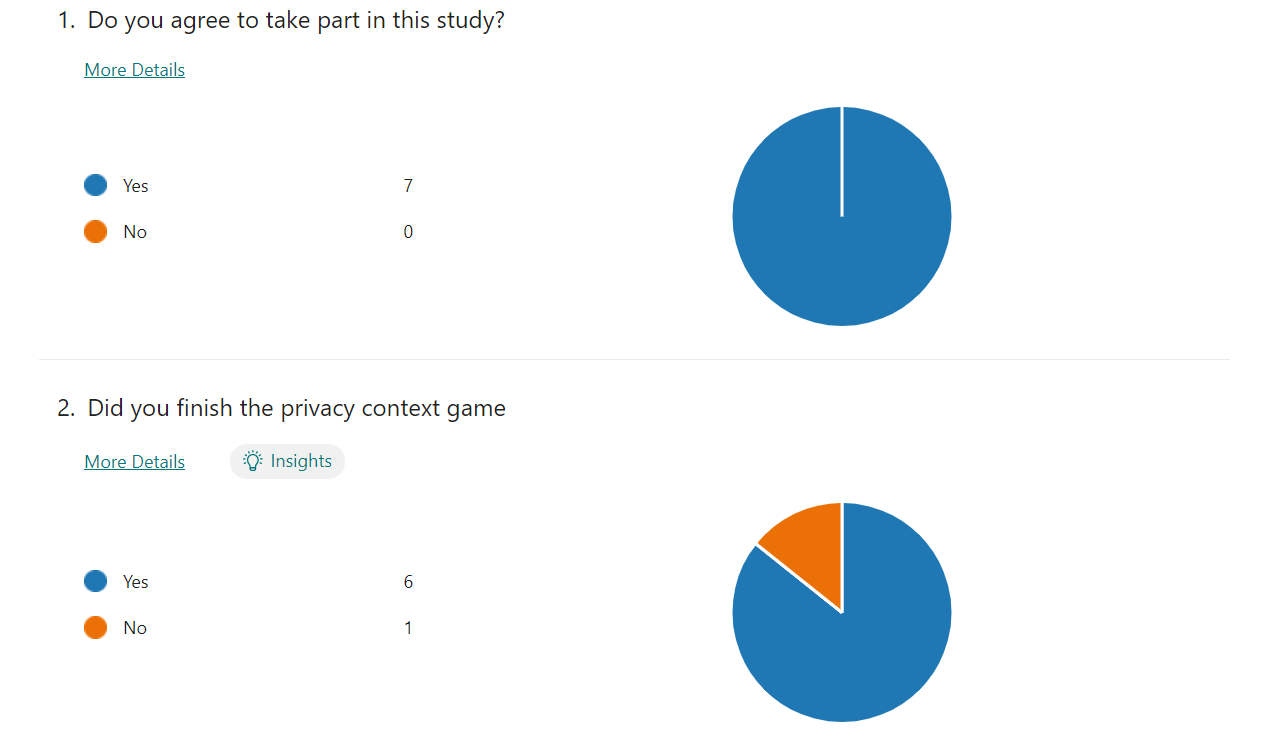
\includegraphics[width=1\textwidth]{Survey1.png}
%width相加大于1时自动换行
%自行调整width \vsapce \hspace
\end{minipage}
}\hspace{-1pt}%调整subfigure的间距
\subfigure[completion time]{
\label{fig:completion}
\begin{minipage}[c]{0.485\textwidth}
\centering
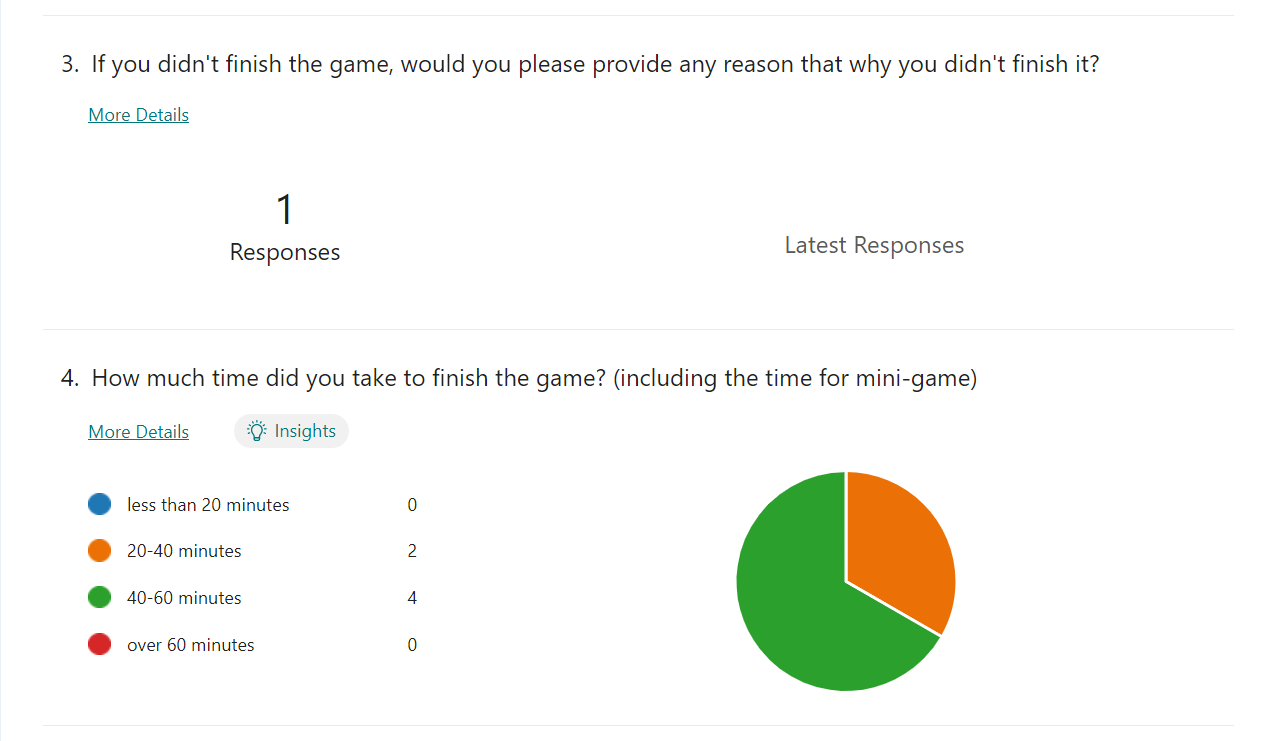
\includegraphics[width=1\textwidth]{Survey2.png}
\end{minipage}
}\hspace{-1pt}%在这里空一行会强制subfigure换行
\caption{Game experience survey part 1}
\label{fig:surveyPart1}
\end{figure}

The survey has a total of 16 questions with different branches. In figure \ref{fig:surveyPart1}, we could find that all seven participants agreed to participate in this study. However, one participant did not finish our game, and the reason was provided in question 3: there were too many questions in this game, which cost time beyond expectation. The overall completion time for the other six participants, including the mini-game, is shown in figure \ref{fig:completion}. All of them completed the game within one hour.

\begin{figure}[htbp]
\center
\subfigure[feedback]{
\label{fig:feedback}
\begin{minipage}[c]{0.485\textwidth} %自行调整,太大的话会自动换行
\centering
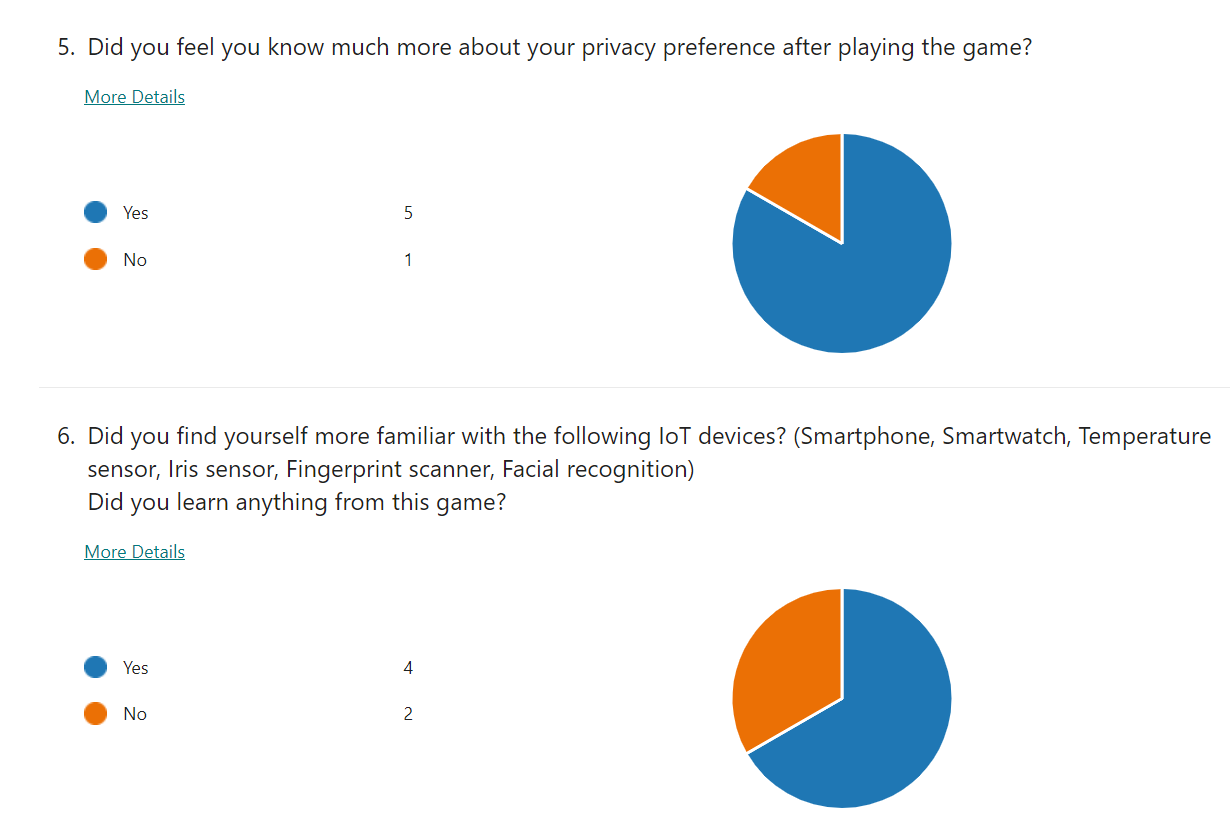
\includegraphics[width=1\textwidth]{Survey3.png}
%width相加大于1时自动换行
%自行调整width \vsapce \hspace
\end{minipage}
}\hspace{-1pt}%调整subfigure的间距
\subfigure[game tutorial and interface]{
\label{fig:tutorial&interface}
\begin{minipage}[c]{0.485\textwidth}
\centering
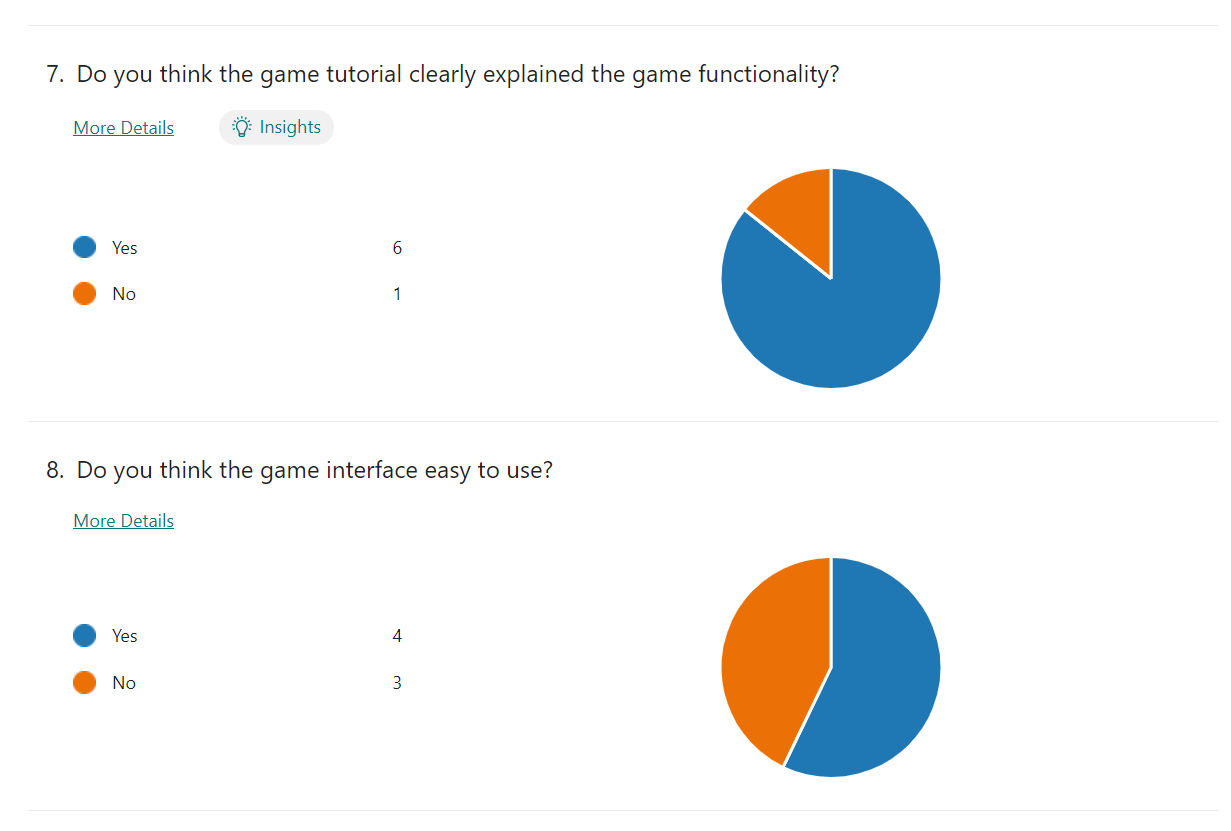
\includegraphics[width=1\textwidth]{Survey4.png}
\end{minipage}
}\hspace{-1pt}%在这里空一行会强制subfigure换行
\caption{Game experience survey part 2}
\label{fig:surveyPart2}
\end{figure}

For participants who completed the game, we asked them two questions regarding two project aims introduced in section \ref{section:aim}, as shown in figure \ref{fig:feedback}. Almost all participants feel they learned more about their privacy preferences, and two-thirds feel they are more familiar with the IoT devices involved in the game. Questions 7 and 8 in figure \ref{fig:tutorial&interface} aim to evaluate the clarity of the game tutorial and interface. The result indicates that we did well on the game tutorial, but the game interface remains to be improved.

\begin{figure}[htbp]
\center
\subfigure[pop-up quiz]{
\label{fig:surveyforquiz}
\begin{minipage}[c]{0.485\textwidth} %自行调整,太大的话会自动换行
\centering
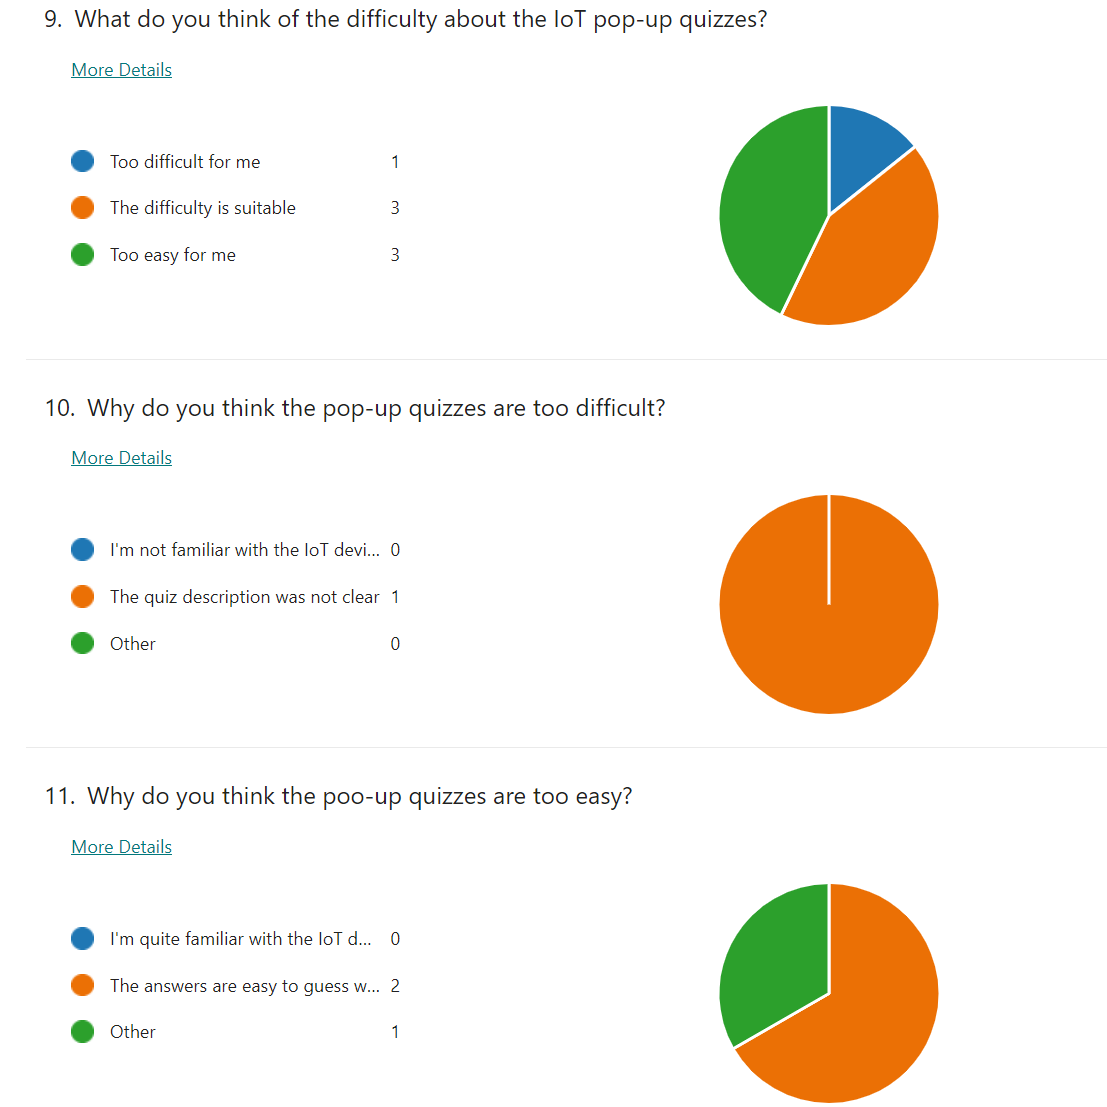
\includegraphics[width=1\textwidth]{Survey5.png}
%width相加大于1时自动换行
%自行调整width \vsapce \hspace
\end{minipage}
}\hspace{-1pt}%调整subfigure的间距
\subfigure[mini-game]{
\label{fig:surveryformini-game}
\begin{minipage}[c]{0.485\textwidth}
\centering
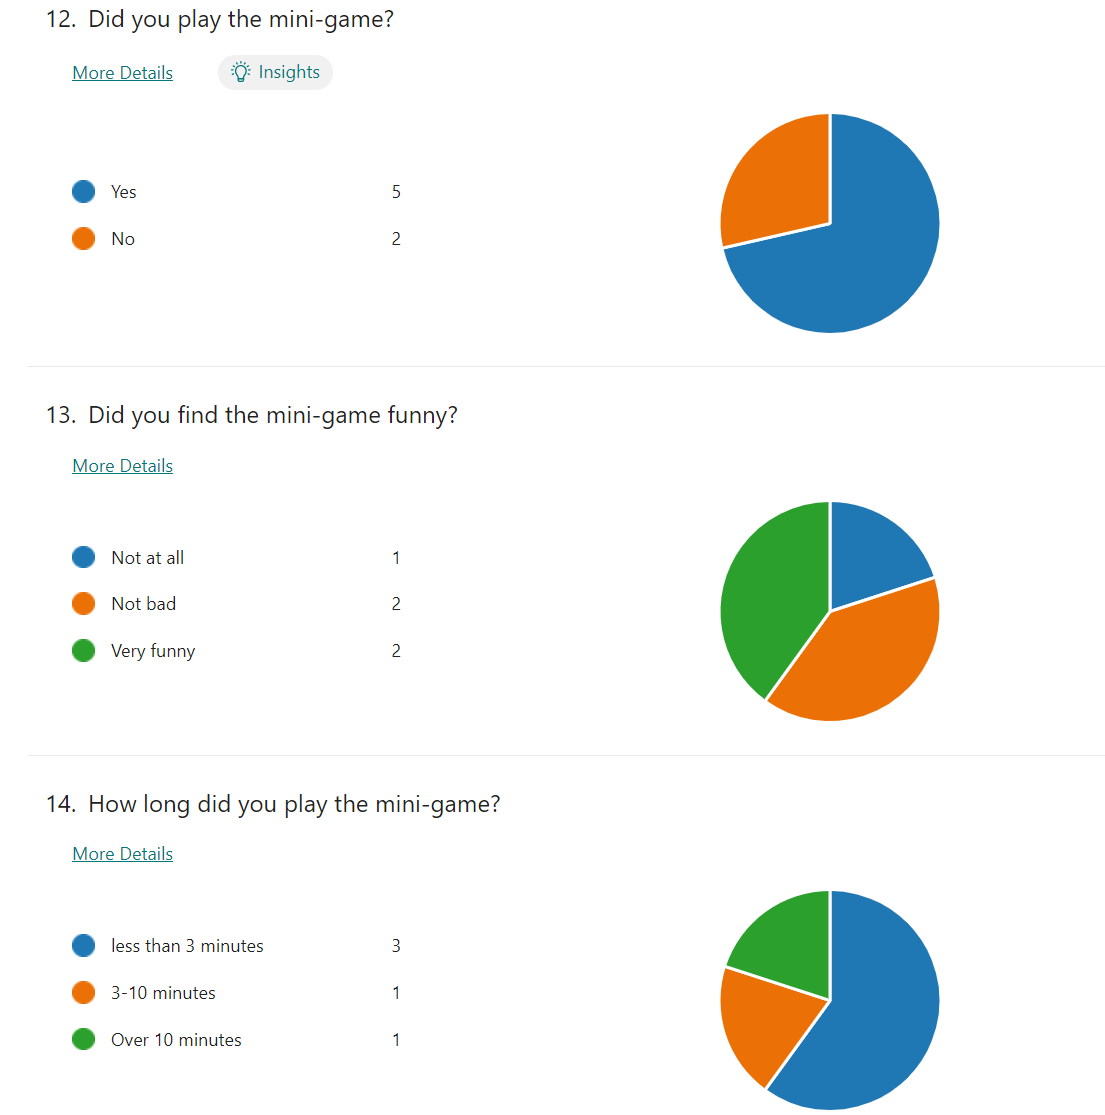
\includegraphics[width=1\textwidth]{Survey6.png}
\end{minipage}
}\hspace{-1pt}%在这里空一行会强制subfigure换行
\caption{Game experience survey part 3}
\label{fig:surveyPart3}
\end{figure}

Figure \ref{fig:surveyforquiz} and \ref{fig:surveryformini-game} are questions for evaluating the pop-up quizzes and the mini-game. All participants took the quizzes, and nearly half thought the quizzes were too easy. According to their feedback, it is partially due to our statements for the quizzes. The hints we gave players are so obvious that they could guess the correct answers without prior knowledge about the IoT devices. Nevertheless, our primary target is to educate players rather than make things difficult. For the evaluation of the mini-game, five participants did try it on, and their evaluations were that the mini-game was better than average. It is worth noting that one participant enjoyed the mini-game for more than ten minutes. It represents that this mini-game has good playability.

\begin{figure}[htbp]
    \centering
    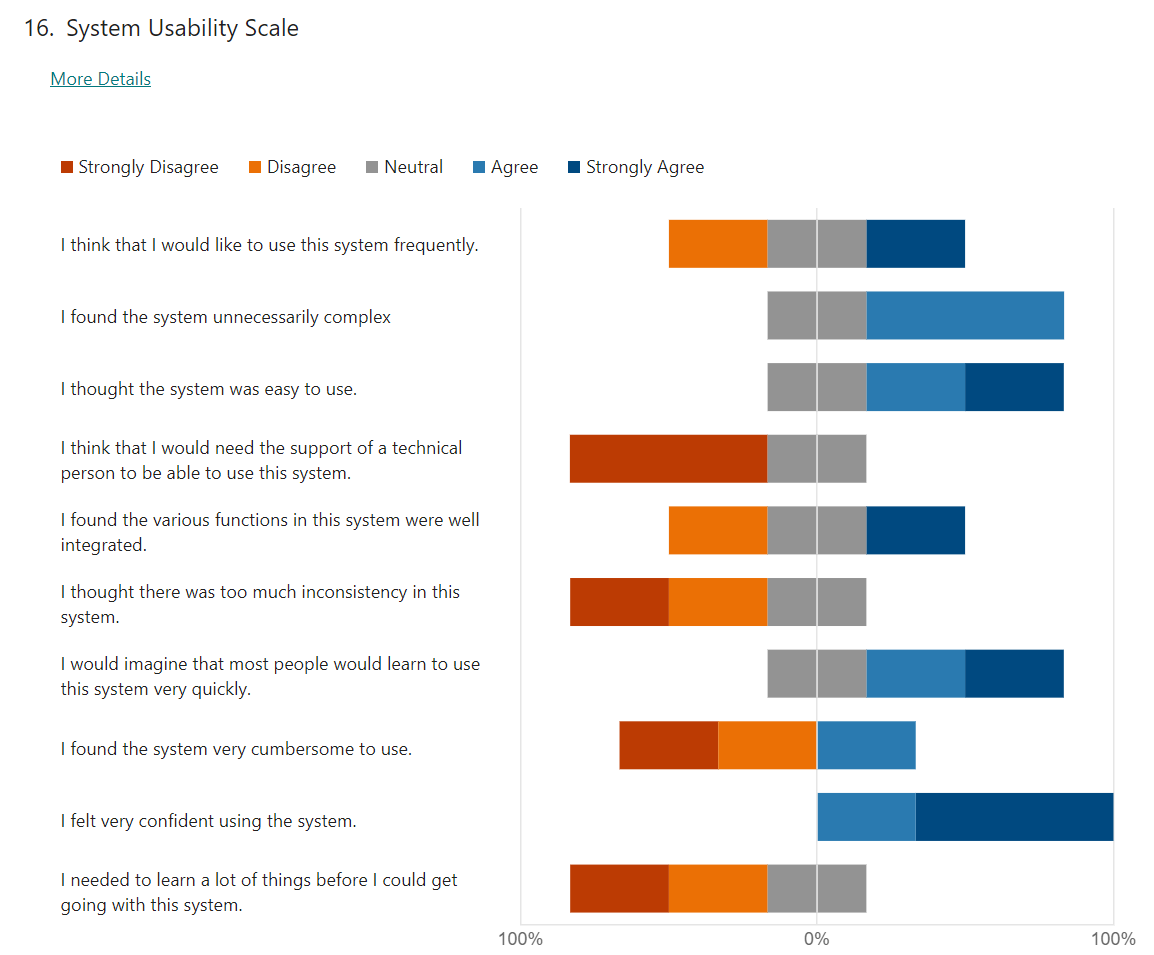
\includegraphics[width=0.8\textwidth]{Survey7.png}
    \caption{System Usability Scale (SUS)}
    \label{fig:SUS}
\end{figure}

The last part of the game experience survey is a system usability scale (SUS). The SUS has been a quick method to evaluate the usability of different human-agent systems and software for almost 20 years\cite{Peres2013ValidationOT}. We received five evaluations from participants for the SUS. According to figure \ref{fig:SUS}, some participants considered the system unnecessarily complex, but they also thought it was easy to use. They also believed that most people would quickly learn to use this system. In the aspect of functionality, various functions in this system were integrated well and consistently.

\section{Further Study}

Participants who have completed the game also uploaded their saved data files to the OneDrive cloud as indicated in the instructions. Subsequently, we downloaded their data files and did some analysis. We have some interesting findings and we will briefly summarize the results.

\begin{itemize}
    \item The importance of factors affecting comfort levels and that of factors affecting decisions are highly consistent, which means if people are more comfortable with the data collection, they are more likely to approve that collection.
    
    \item We found that participants changed their minds in two consecutive scenarios in which only one factor changed. We conclude that it is conducive to determining privacy preferences if we compare two similar scenarios.
    
    \item Almost every one gets 100\% grade on the pop-up quizzes, and the numbers of tries on each quiz are small. Some participants used tips to improve their accuracy.
\end{itemize}

\chapter{Conclusion}

In this project, we used the Unity engine to build an educational game that helps players learn about their privacy preferences and become more familiar with IoT devices. We firstly designed 75 scenarios of data collection in which players would face in the game and make their choices on comfort levels and decisions regarding different scenarios. To incorporate education with entertainment, we designed a pop-up quizzes system with tips and embedded a mini-game into our project to motivate players to achieve higher grades on the quizzes. We stored players' information in JSON files such that their game sessions could be restored. We also built two statistical models for analyzing the importance of factors by calculating Spearman's rank correlation coefficients. The results are shown in pie charts and bar charts to better visualize each factor's effect. Additionally, players' performances on pop-up quizzes and their personal feedback for IoT devices are also provided in the results pages.

We conducted a user study after the implementation of the game to evaluate the game and the system's usability. According to the game experience survey, we received good grades on the System Usability Scale, and two primary project aims were also achieved. However, we also need to improve the design of pop-up quizzes and the game interfaces. Furthermore, we studied saved game files uploaded by participants and had exciting findings. These findings could give us insights into designing better educational games in future.

Although there are still limitations to the project, and many aspects remain to be improved, we are informed and gained experience through this project. In summation, we successfully achieved our tasks, and we believe this project will profoundly impact us in researching individuals' privacy preferences and developing future educational games.

% The body of your dissertation, before the references and any appendices,
% \emph{must} finish by page~40. The introduction, after preliminary material,
% should have started on page~1.

% You may not change the dissertation format (e.g., reduce the font
% size, change the margins, or reduce the line spacing from the default
% 1.5 spacing). Over length or incorrectly-formatted dissertations will
% not be accepted and you would have to modify your dissertation and
% resubmit.  You cannot assume we will check your submission before the
% final deadline and if it requires resubmission after the deadline to
% conform to the page and style requirements you will be subject to the
% usual late penalties based on your final submission time.

\bibliographystyle{plain}
\bibliography{mybibfile}

%% You can include appendices like this:
\appendix

\chapter{Participant Information Sheet}
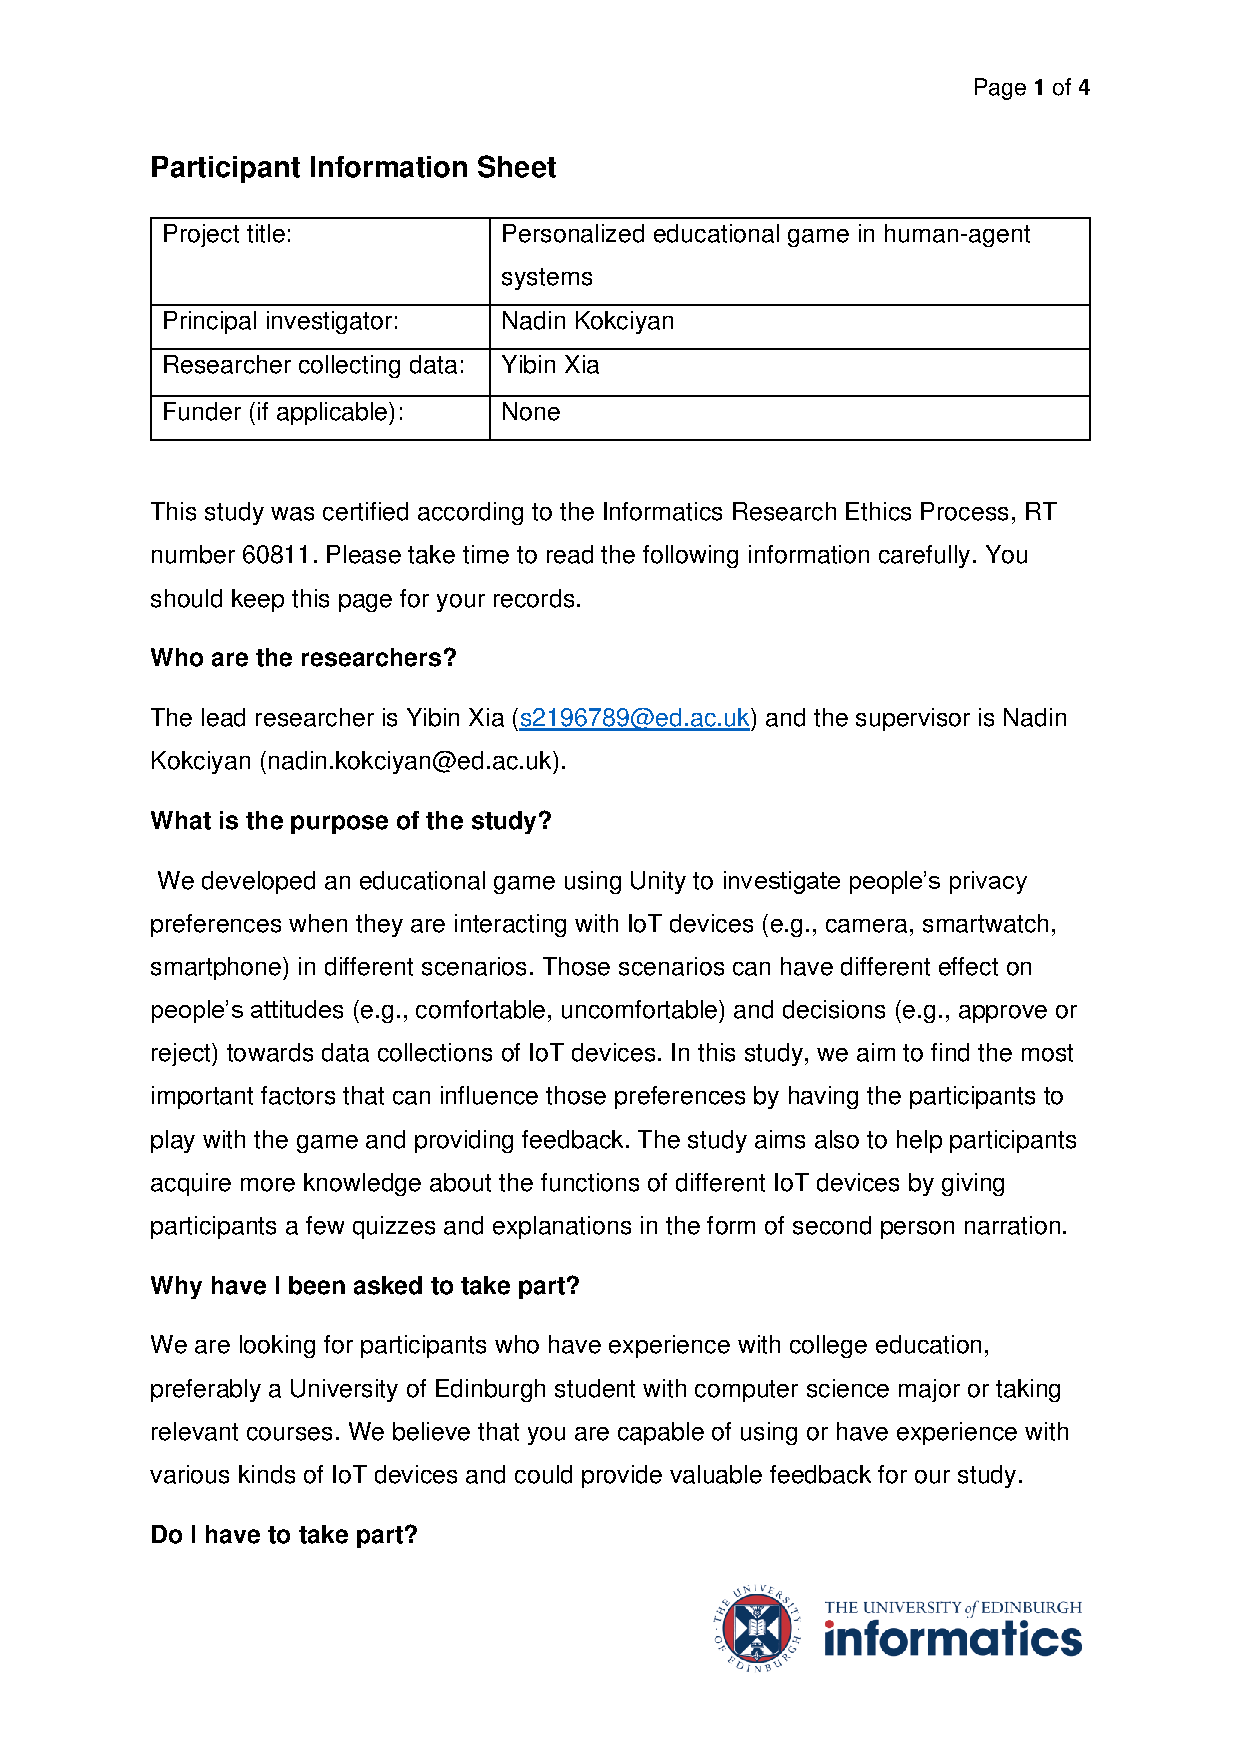
\includepdf[pages=-]{PIS.pdf}

\chapter{Game Experience Questionnaire}
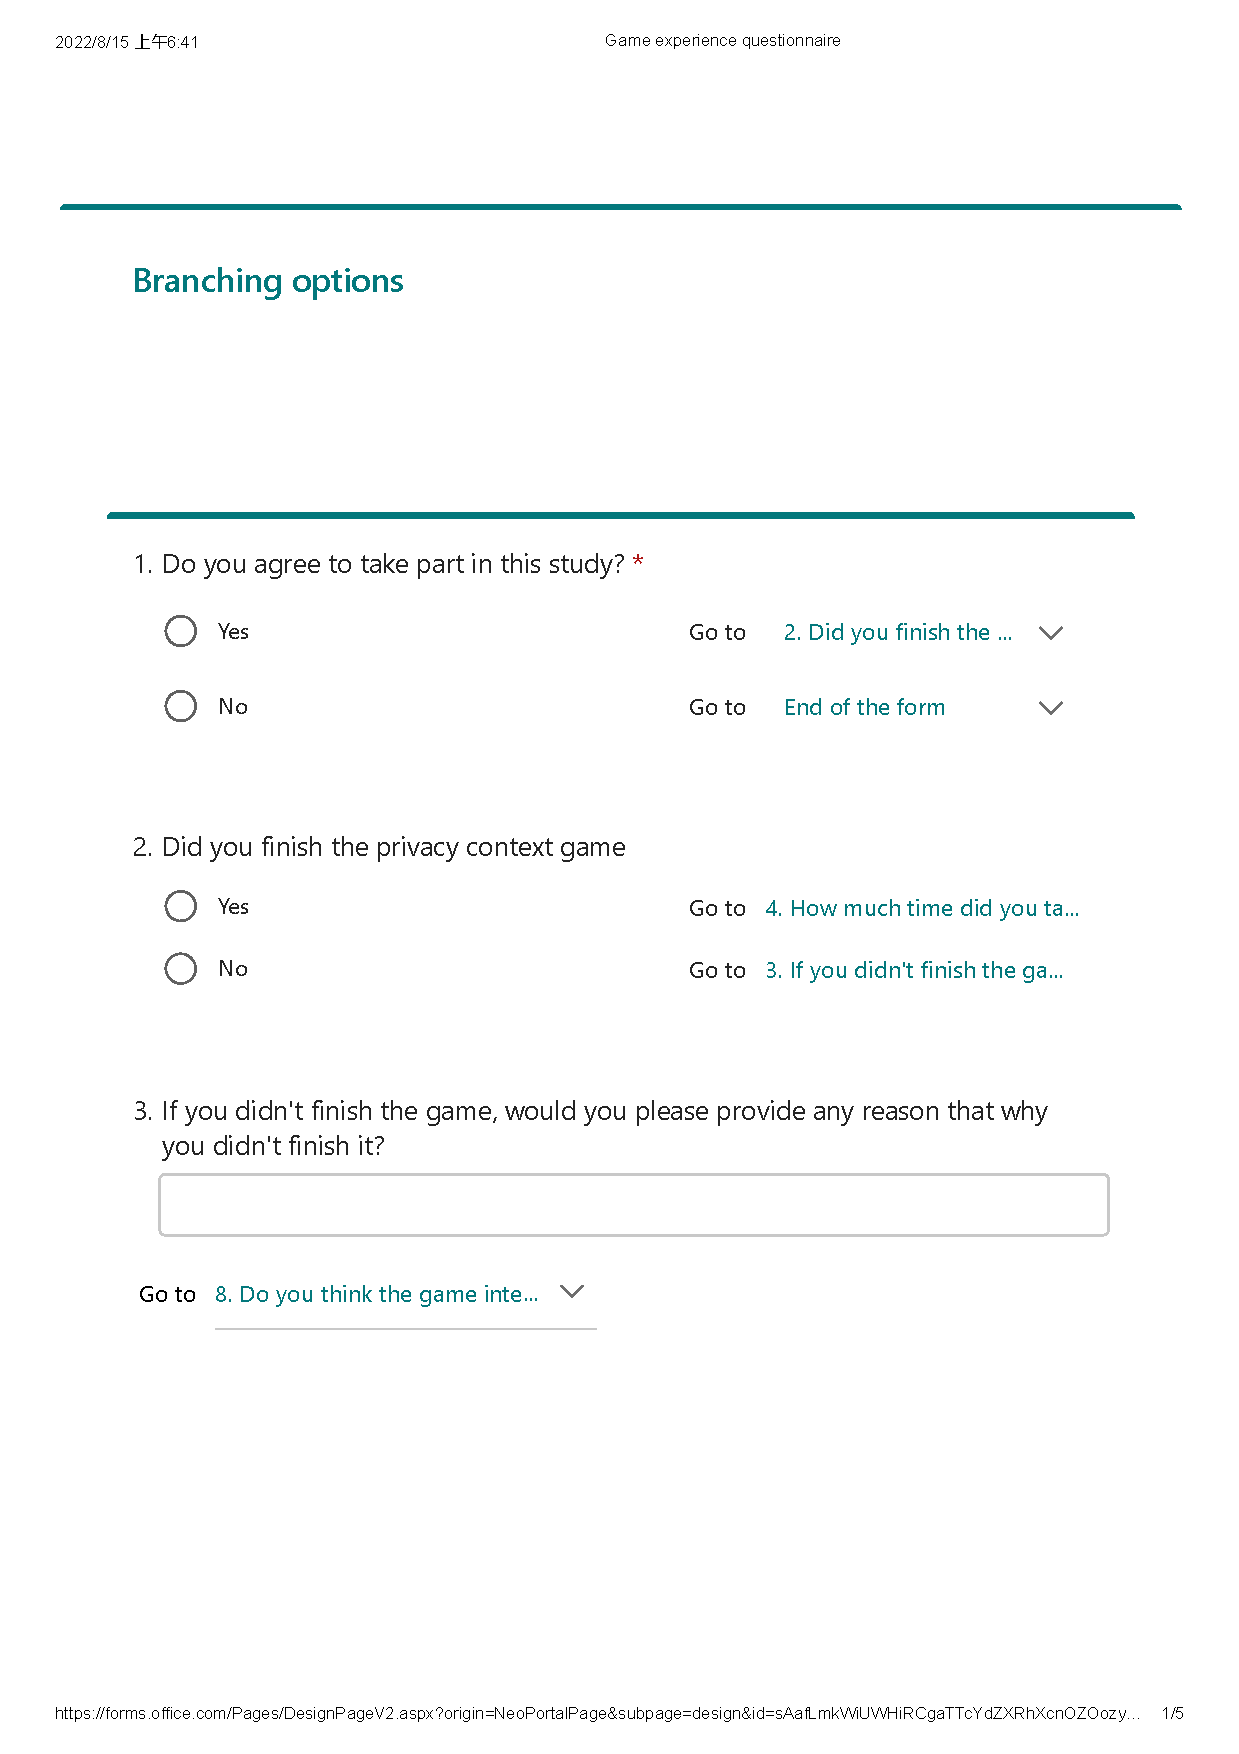
\includepdf[pages=-]{Game experience questionnaire.pdf}

% Markers do not have to consider appendices. Make sure that your contributions
% are made clear in the main body of the dissertation (within the page limit).

\end{document}
